\documentclass[final,subfig,blackref]{drexel-thesis}

\usepackage{amsmath}
\usepackage{amsthm}
\usepackage{amssymb}
\usepackage{esvect}

\usepackage{pdflscape} % For the observational data table
\usepackage{longtable} % For the observational data table

\usepackage{natbib}
\bibliographystyle{yahapj}

\usepackage{aastex_hack}

%% For uncommon journals
%\newcommand\mnras{{MNRAS}}%
%\newcommand\aap{{A\&A}}%
%\newcommand\aaps{{A\&AS}}%
%\newcommand\apj{{ApJ}}%
%\newcommand\apjl{{ApJ}}%
%\newcommand\apjs{{ApJ}}%
%\newcommand\araa{{ARA\&A}}%
%\newcommand\aj{{AJ}}%
%\newcommand\ssr{{Space Sci. Rev.}}%
%\newcommand\pasj{{PASJ}}% 
\newcommand\nar{{NAR}}%
%\newcommand\physrep{{Physics Reports}}%


\author{Austen M. Groener}
\title{Dark Matter in Galaxy Clusters: Shape, Projection, and Environment}
\DUTmonth{September}
\DUTyear{2015}
\degree{Doctor of Philosophy}
\advisor{Dr. David Goldberg}
\copyrighttext{}

\begin{document}

\begin{preamble}

\iffinal{}{\newpage}
\begin{DUTdedications}
%
\vspace*{\fill}
%
\begin{center}
\setstretch{2}
\begin{minipage}{8 cm}
\begin{center}
\hrulefill\\
This thesis is dedicated to Cara Hoppe.\\ 
I respect her as my peer,\\
and cherish her as my wife.\\
Her love and support made this work possible. \\
%\hrulefill\hspace{0.2cm} \leafNE \hspace{0.2cm} \hrulefill
\hrulefill
\vspace{6em}
\end{center}
\end{minipage}
\end{center} 
%
\vspace*{\fill}
%
\end{DUTdedications} 
\iffinal{}{\newpage}

\begin{acknowledgments}
  \iffinal{}{\setstretch{1.5}}
The completion of this thesis could not have been done without the tireless support of my advisor, Dr. Jian-Min Yuan. I am deeply indebted for the support he has provided over the years. As a mentor, he helped me develop my skills as a scientist and honed my critical thinking. He is an endless source of new ideas and has taught me how to effectively communicate in the scientific world. 

I would also like to thank the physics department at Drexel for helping me prepare for the journey ahead. In particular, both Dr. Michel Vallieres and Dr. Robert Gilmore have been gracious enough to spend many afternoons discussing every interesting theory I've come across. Their insights and enthusiasm for physics and mathematics is inspiring. 

I would like to thank my family, my wife, Cara Hoppe, and my children, Hazel and Jackson Hoppe. They cheerfully remind me of the world outside and always bring a smile to my face. Finally, I would like to thank my uncle, Fred Stein, who introduced me to physics and all its wonders at an early age.
 
  \end{acknowledgments}
  \iffinal{}{\newpage}

  \listoffigures 
  \iffinal{}{\newpage}

  \tableofcontents 
  \iffinal{}{\newpage}

  \begin{abstract}
  \iffinal{}{\setstretch{1.5}}
  \setstretch{1.5}
A protein's ultimate function and activity is determined by the unique three-dimensional structure taken by the folding process. Protein malfunction due to misfolding is the culprit of many clinical disorders, such as abnormal protein aggregations. This leads to neurodegenerative disorders like Huntington's and Alzheimer's disease. We focus on a subset of the folding problem, exploring the role and effects of entropy on the process of protein folding. Four major concepts and models are developed and each pertains to a specific aspect of the folding process: entropic forces, conformational states under crowding, aggregation, and macrostate kinetics from microstate trajectories. 

The exclusive focus on entropy is well-suited for crowding studies, as many interactions are non-specific. We show how a stabilizing entropic force can arise purely from the motion of crowders in solution. In addition we are able to make a a quantitative prediction of the crowding effect with an implicit crowding approximation using an aspherical scaled-particle theory.

In order to investigate the effects of aggregation, we derive a new operator expansion method to solve the Ising/Potts model with external fields over an arbitrary graph. Here the external fields are representative of the entropic forces. We show that this method reduces the problem of calculating the partition function to the solution of recursion relations. 

Many of the methods employed are coarse-grained approximations. As such, it is useful to have a viable method for extracting macrostate information from time series data. We develop a method to cluster the microstates into physically meaningful macrostates by grouping similar relaxation times from a transition matrix.  

Overall, the studied topics allow us to understand deeper the complicated process involving proteins.
  \end{abstract} 

	\iffinal{}{\newpage}

\end{preamble}


\begin{thesis}
  \pdfbookmark[-1]{Main Matter}{Main Matter}
  \ifdaring{\setstretch{1.3}}{}
  %\ifdaring{\setstretch{1.3}}{\setstretch{1.3}}
  
  %CHAPTER: Introduction
  \chapter{Introduction}

The practice of staining glass for decorative purposes dates to ancient Rome,
but the investigation of light matter interaction starts even back to the
begining of history for human beings, when ancient men wondered about the
source of light ,sun, or the first time to use a torch for hunting. People
never stop studying how the light interacts with our world, meanwhile, this
leads to improving our understanding and building a better world with photonic
technology. The stained-glass windows such as the one inside of the St.
Patrick's Cathedral in Fig.~\ref{StainGlass} served as a 'poor man's Bible' in
the Middle Ages, allowing believers who could not read Latin to learn the story
of the Gospels.  The term stained glass refers to glass that has been coloured
by adding metallic salts during its manufacture. Then this coloured glass is
crafted into stained glass windows in which small pieces of glass are arranged
to form patterns or pictures. Even nowadays, people are still surprised about
how beautiful they are and wondering how the light interact with these pieces
of art crafts. Besides the arts, lighting technology is also evolving very
rapidly, from the ancient torchs to the bulb that Thomas Edison invented and to
the modern LEDs such as the ones also shown in Fig.~\ref{StainGlass}. From
blackbody radiation to electroluminescence, i.e., from thermal radiation to
radiative recombination, we are now capable of generating light more
efficiently.

\begin{figure}
  \caption{The Stained-glass window and the top modern lamps inside of the St. Patrick's Cathedral, 5th Ave, New York, NY.}
  \centering
  \includegraphics[width=0.5\textwidth,height=0.5\textheight]{pictures/Introduction/StainGlass}
  \label{StainGlass}
\end{figure}

Now we find ourselves living through a new revolution in the age of information
technology, one with consequences every bit as dramatic and likely even more
profound as the data transmission by light. Electrons have served us very well
for the past few decades, but the explosion of data. The storage and the
transmission of data consumes large amount of power and time, simultaneously.
Meeting the energy needs of the communication of information, together with
storage and computation form a "grand challenge" of the information age.

One good example of huge amount of power consumption by data transmission and
computation is the data centers, which currently consume 1.5\% of global energy
production, and up to approximately 4\% of U.S. energy produced. Though the
statistics seems small, a 1000 times increase in the volume of data is
predicted by 2025~\cite{Hilbert:2011tg}. Google data center alone consumes
enough electricity to power 200,000 homes, since an average Google search or a
YouTube video or a message through Gmail uses 0.3 watt-hours of
electricity~\cite{glanz2011google}. Having efficient data computation and
transmission tools will greatly reduce the total data center power consumption
into a greener number. And the data pipelines of light can certainly be very
helpful in this regime.

\section{Background} \label{sec:intro_BG}

\subsection{Photonics and Optoelectronics}

Photonics involves the generation, control and detection of lightwaves and
photons, which are particles of light, in free space or solid.
Optoelectronics is the study and application of effects related to the
interaction of light and electronic signals, and may be considered a sub-field
of photonics. Both photonics and optoelectronics study the light, and explore a
wider variety of wavelengths besides visible lightwave range, from gamma rays
to radio, including X-rays, ultraviolet and infrared light.

The invention and development of solar
cells~\cite{sun2005organic,perlin1999space},
photodetector~\cite{razeghi1996semiconductor,rogalski2002infrared},
modulators~\cite{chen2011broadband,schuller2010plasmonics},
LEDs~\cite{spanggaard2004brief,schubert2005solid,schubert2005light} and
lasers~\cite{chow2012semiconductor,yablonovitch1987inhibited} certainly set the
example of breakthroughs due to the manipulation of photons in thin films and
semiconductor bulk crystals. The continuing success of photonic technologies
relies on the discovery of new optical materials and the miniaturization of
optoelectronic devices that feature better performance, low cost and low power
consumption. For the last few decades, countless efforts in nano-scale
materials and devices research have created a rich collection of nanostructures
where size, shape and composition can be readily controled. Many such
nanostructures exhibit fascinating optical properties that could have
significant impact in the future for photonic technology.

\subsection{Core-Shell Nanowires} \label{sec:intro_CSNW}

The primary principle for constantly miniaturizing the device is not only about
the size, but also to have better electronic and optical properties. As the
critical dimension of semiconductor solid-state devices keep shrinking, the
effect of charge carriers quantization becomes more prominent, and to be more
specific, this means the confinement of electrons or holes by constructing
quantum confined structures. At the very dawn of electronics, the idea of using
heterostructures (i.e., the structure with two layers or regions of dissimilar
crystalline semiconductors) has emerged. After Shockley proposed the idea,
Alferov and Kroemer introduced the concept that heterojuctions could possess
high injection efficiencies in comparison with homojunctions, and which we know
now is due to the confinement of carriers~\cite{alferov2000double}. It would be
very difficult today to imagine solid-state physics without semiconductor
heterostructures for both electronic-based and optical-based applications. The
heterostructures and, especially, double heterostructures, including quantum
wells, nanowires, and quantum dots, are the fundamental building blocks for
current nanoscience research as depicted in Fig.~\ref{Nanomaterials}.

\begin{figure}
  \caption{Diagram of classification of nano-materials and nano-scale structures}
  \centering
  \includegraphics[width=\textwidth]{pictures/Introduction/Nanomaterials}
  \label{Nanomaterials}
\end{figure}

Quantum well is a potential well which confines particles to only move freely
in two dimensions in stead of three dimensions, by forcing them to occupy a
planar region. These wells are typically formed in semiconductors by having a
narrower bandgap material sandwiched between two layers with wider bandgap
materials. Electrons in quantum wells are confined in two dimensions either
naturally or by doping the barrier of a quantum well, thus a two-dimensional
electron gas (2DEG) may be formed at the heterointerface. This not only
increases the density of electrons, but also causes a better performance in
optoelectronic devices such as laser diodes~\cite{nakamura1996ingan}, High
Electron Mobility Transistors (HEMTs)~\cite{kuzmik2002inaln,rosenberg19850},
photodetectors~\cite{levine1993quantum,liu2004terahertz}, and solar
cells~\cite{barnham2002quantum,ekins1999strain}.

Quantum dots, as another most common nanostructure in semiconductor physics,
exhibit much more enhanced optical properties. They are normally only several
nano-meters in size, and either synthesized or self-assembled into a bulk
solid. As the particles in the quantum dots are confined in three dimensions,
which leave them zero degree of freedom. As a result, the density of states
changes to a delta function as opposed to a smooth square root dependence that
is found in bulk materials. The narrower peak spectra and larger magnitude of
intensity make them even better candidates in the application of solar
cells~\cite{nozik2002quantum},
lasers~\cite{klimov2000optical,ustinov2003quantum} and light emitting diodes
(LEDs)~\cite{park2001band,sun2007bright}.

However, since the introduction in the 1990's, another important class of
semiconductor nanostructures has emerged: structures with cross-sections of
tens or hundreds of nano-meters and lengths up to several micro-meters. These
structures are named as 'nanowires'~\cite{xia2003one} different from quantum
dots as they are confined only in two dimensions, thus allowing electrons,
holes or photons to propagate freely along the third dimension. Besides their
own outstanding electro-optical properties, the high-aspect-ratio of these new
semiconductor nanostructures allows for the bridging of the nanoscopic and
macroscopic world. As P. Yang writes in their review paper:~\cite{Yan:2009hm}
"This nano-macro interface is fundamental to the integration of nanoscale
building blocks in electrical or optoelectronic device applications.
Conventional photonic platforms often consist of features with large
aspect-ratios such as interconnects and waveguides, typically with micrometre
dimensions. Thus, when semiconductor nanowires emerged they were immediately
recognized as one of the essential building blocks for nanophotonics."

The development of sophisticated nanowires growth
techniques~\cite{hobbs2012semiconductor,wu2001direct}, either
bottom-up~\cite{lu2007nanoelectronics,Huang:2001kv} or
top-down~\cite{park2009top}, has stimulated a large body of new work in
semiconductor nanowires over the last twenty years or so. Previously, the
research activities focused on the growth of higher quality
nanowires~\cite{Yang:2002ts} and the variation of its constituent materials. At
that time, most of the nanowires were core-only with ZnO~\cite{Yang:2002ts},
GaAs~\cite{persson2004solid}, Si~\cite{hochbaum2005controlled}, or
Ge~\cite{wu2000germanium}. However, later on, researchers found out that
growing an additional layer of shell can increase quantum yield by passivating
the surface trap states. In addition, the shell provides protection against
environmental changes, photo-oxidative degradation, and provides another route
for modularity. Precise control of the size, shape and composition of both the
core and the shell enable engineering the device with many degree of freedom
and optoelectronic properties, such as the tuning of the emission wavelength
over a wider range of wavelengths than with either individual semiconductor.
Undoubtedly, much of this interest was further stimulated by the possibility of
novel physics and applications in core-shell nanowires.

The successes of semiconductor nanowires in optoelectronics and the promising
physical mechanisms using quantum-confined structures have, furthermore,
enlivened the debate over possible applications of optics for functions such as
transmission, logic and switching in communications and computation. It is
important to emphasize at the outset that quantum confinement produces not only
quantitative but also qualitative differences in physics compared to that in
bulk structures, which is of course another major motivation for the interest
in them. As Dr. Miller discussed in the paper about quantum
well:~\cite{schmitt1989linear} "There are many examples of these differences.
The optical absorption spectrum breaks up into a series of steps associated
with the quantum-confined electron and hole levels. Excitonic effects become
much stronger because of the quantum confinement, giving clear absorption
resonances even at room temperature. The relative importance of direct Coulomb
screening and exchange effects is quite different in quantum wells (the Coulomb
screening is relatively much weaker), giving very different optical saturation
behaviour." Similar to quantum wells, nanowires have been observed to have even
more profound differences in physics. Thus, the analysis and discussion about
different behavior of nanowires and bulk semiconductors when they interact with
light will be the primary topic of this dissertation.

\section{Literature Review} \label{sec:intro_LR}

Since the introduction of initially so-called 'nanowhiskers' in the
1990s~\cite{yazawa1991heteroepitaxial}, semiconductor nanowires have been
extensively studied and much insight has been gained on tuning their electrical
and optical properties. Nanowire related articles have shown a healthy increase
in number published from 2005 to 2016, as Fig.~\ref{ISIPublication} (blue bars)
shows. Article with topics on optical properties of nanowires comprise a good
portion in all the nanowire-related papers published in the recent decade,
showing clear increasing trend in the number of papers on NW optics or
photonics (green bars), presently comprising more than four-fifth of the
nanowire-related articles.

\begin{figure}
  \caption[Article with topics on optical properties of nanowires consist of a large portion of all the nanowire-related papers published from 2005 to 2016.]{Article with topics on optical properties of nanowires consist of a large portion of all the nanowire related papers published from 2005 to 2016. (Source: ISI website, keyword: Nanowire (blue), Nanowire AND optical OR optoelectronic OR photonics (grey))}
  \centering
  \includegraphics[width=\textwidth]{pictures/Introduction/ISIPublication}
  \label{ISIPublication}
\end{figure}

The applications and classifications of NWs are shown in
Fig.~\ref{NWApplication}. In terms of the geometric strcuture, the most common
NWs are cylindrical~\cite{Cao:2010dc,Cao:2009ho} and
hexagonal~\cite{Royo:2015vw,Currie:2013to} due to the growth techniques. And as
discussed previously, there are
core-only~\cite{Heo:2004fp,he2007piezoelectric,Duan:2003en},
core-shell~\cite{Moratis:2016ws,Wang:2015bz} and
core-multi-shell~\cite{Badada:2015jq,Takehiro:2016tl} configurations in order
to exploit various properties of NWs. In addition, NWs have been used as
electronic based devices, such as High Electron Movement Transistors
(HEMTs)~\cite{li2006dopant,sakaki1980scattering}, Field Effect Transistors
(FETs)~\cite{xiang2006ge,singh2006high,suk2005high},
capacitors~\cite{Liu:2012cz}, diodes~\cite{Wallentin:2010kf,heo2004pt},
and optoelectronic based devices, such as
lasers~\cite{Li:2015ir,Wei:2014hr,Saxena:2013fe,Mayer:2013jh,Chen:2011cg,Hua:2009kf,Agarwal:2005is,Gradecak:2005eb,Duan:2003en},
LEDs~\cite{Zhao:2015hl,Nami:2015df,Chuang:2011jk,Bavencove:2011io,Kim:2004je},
Solar Cells~\cite{Wang:2015dp,Yu:2014hj,Wang:2012dh,Kelzenberg:2010fa,Garnett:2008jk,Tsakalakos:2007kz,Tian:2007kl},
Photodetectors~\cite{Chen:2015dz,deLunaBugallo:2010ci,Cao:2010dc,Pettersson:2006ft,Kind:2002fk,Liang:2001ka},
waveguides~\cite{Grego:2011ka,Oulton:2008fi,Yamada:2005bl,Sirbuly:2005ir,Chandrasekhar:1987kk},
phototransistors~\cite{Zhang:2010fq,Seo:2010cf,Persano:2010if,Park:2008cn,Logeeswaran:2008fw}.

\begin{figure}
  \caption{Diagram of nanowires applications and classifications}
  \centering
  \includegraphics[width=\textwidth]{pictures/Introduction/NWApplication}
  \label{NWApplication}
\end{figure}


Exciting developments have been made in the academia environment from many
research groups worldwide, including notably the Lieber group at Harvard
University~\cite{Agarwal:2005is,Gradecak:2005eb,Patolsky:2005uz,Duan:2003en,li2006dopant,qian2008multi},
the Yang group at
Berkeley~\cite{Johnson:2003ww,Wu:2002ws,Kind:2002fk,Yang:2002ts,wu2001direct},
the Samuelson group at Lund
University~\cite{Ganjipour:2014cm,Storm:2012gm,Wallentin:2010kf,Thelander:2008uw,Pettersson:2006ft},
and the Wang group at Georgia
Tech~\cite{pan2001nanobelts,wang2006piezoelectric,wang2013nanowires,bae2011fiber,wang2007direct,he2007piezoelectric}.
With different perspectives, these research groups focus on a variation of NW
materials, growth techniques and applications as shown in
Fig.~\ref{NWApplication}. The development of semiconductor NW materials follow
the similar road as bulk materials, from initial single element (e.g.,
Si~\cite{hochbaum2005controlled}, Ge~\cite{wu2000germanium},
Carbon~\cite{zhao2003carbon} et al.) to compound binary
(ZnO~\cite{Johnson:2003ww}, GaN~\cite{Das:2011ci,Gradecak:2005eb},
CdSe~\cite{Persano:2010if}, ZnS~\cite{Ding:2004di}, ZnSe~\cite{xiang2003green},
InP~\cite{Logeeswaran:2008fw}, CdS~\cite{Ding:2004di}, GaAs~\cite{Joyce:2007bl}
et al.), ternary (InGaAs~\cite{Zhao:2014jt}, CdSSe~\cite{pan2006fabrication},
AlGaN~\cite{Li:2015ira}) or even quaternary (AlInGaN~\cite{Wang:2015bi}), then
to currently popular III-V heterostructure NWs(e.g.,
GaAs/AlGaAs~\cite{Peng:2014ia,Wei:2014ws}, GaAs/InGaAs~\cite{Chen:2011ct},
InGaN/GaN~\cite{Zhang:2016tk}, GaAs/GaAsP~\cite{Hua:2009kf} et al.). 

At the same time, many important electronic and optical properties have been
observed, and some of the fundamental applications have been demonstrated as
well. The first optical pumped nanowire laser was demonstrated by the Yang
group~\cite{Huang:2001kv} at 2001, and two years later, the Lieber group showed
the first electrically injected nanowire laser~\cite{Duan:2003en} which makes
NW a potential candidate to be integrated in the electronic-based integrated
circuits.

In the field of industry and commercialization, several companies have started
their adventure in the areas like energy, environment, bio-medicine etc., with
products that influencing our daily life. The glo-USA, Inc.~\cite{GloLED:2017}
is an LEDs manufacturing company at Sunnyvale, CA. They use nanowire arrays
which fabricated on chip to generate light as shown in Fig.~\ref{GloLED}(a).
Each nanowire acts basically as an individual light-emitting diode (LED) with
two circular metal contacts as anode and cathod. The inset is the 45 degree
magnified view of the NW array. Except the fabricated blue nLED as in
Fig.~\ref{GloLED}(b), all color of the visible spectrum, ranging from deep blue
to red, can be realized using nanowire LEDs with industry-standard
semiconductor material and manufacturing equipment.  Since these nanowires are
made using one material system with the active layers grown on the non-polar
plane, they can reduce the wavelength shift and efficiency drop that are
observed with other commercially-available planar LEDs. This will enable a true
white RGB (red, green and blue) LED without the need of lossy phosphor
conversion, thus achieving the highest Color Rendering Index (CRI) and
efficiency.

\begin{figure}
  \caption[Scanning Electron Microscopy image of actual glo nanowire chip and the fabricated blue nLED.]{(a) SEM of actual glo nanowire chip showing magnified 45 degree view of  individual nanowires. (b) The fabricated blue nLED. Each dot represents a nanowire LED. The inset shows top view SEM of nanowire array. Courtesy of glo-USA, Inc.}
  \centering
  \includegraphics[width=\textwidth]{pictures/Introduction/GloLED}
  \label{GloLED}
\end{figure}

From academic research to industrial applications, from efficient electrons
transportation to high quality light confinement, and from applications for
environmental concerns to electronic devices in the daily life, the interaction of
light and nanowires need to be investigated, thus, the major topic of this
dissertation is to study the optoelectronics properties of core-shell nanowires
and how they interact with light when electrons in this nano-scale structure
are confined to lower dimensionality.

\section{Scope and Organization of the Dissertation}

This thesis is structured as follows. The growth techniques and electro-optical
properties of core-shell nanowires are presented in Chapter~\ref{data}.  After
introducing four different light confinement mechanisms, i.e., Leaky Mode
Resonance, Whispering Gallery Modes, Fabry-Perot Resonant Mode and Helical
Resonance Modes, Chapter~\ref{LM} presents our findings for a generalized
volumetric modes with light management of sub-wavelength cavities.
Chapter~\ref{ED} presents our methods and findings for calculating band-bending
and electronic distribution in both cylindrical and hexagonal core-shell
nanowire by solving Poisson-Schrodinger equations self-consistantly.  In
Chapter~\ref{RM}, we apply the inter-band optical transition rates study to
understand the extremely enhanced optical properties of hexagonal core-shell
nanowires, and identify three primary factors (overlap integral, oscillator
strength and joint optical density of states) which are strong function of
dimensionality. The quantum mechanical derivation based on perturbation theory
and Fermi's Golden Rule used in this chapter are outlined in more detail in
Appendix~\ref{ch:rates}. The modeling of lasing threshold based on the optical
transition rates in Chapter~\ref{LT} confirmed that our theoretical
explanation, analysis and calculation of optical properties of core-shell
nanowire have a very strong dependence on electron confinement. Finally, we
present our conclusions in Chapter~\ref{conclusions}.

Throughout this work we use the term  {\em nanowires} (NWs) to represent a
specific quantum confined structure with cross-sections of 2-300 nm and lengths
upwards of several micrometers. There are other research groups using terms
such as {\em nanopillars}, {\em nanotubes} or {\em quantum well wires} (QWRs)
to discuss the same nanostructures.

  
  %CHAPTER: Work In Simulations and Theory
  \chapter[Cluster Shape and Orientation]{Shape Profiles and Orientation Bias for Weak and Strong Lensing
  Cluster Halos}

\section{Introduction}

Gravitational lensing has proven an incredibly useful tool in
creating detailed maps of projected density without requiring any
assumptions regarding either a halo's dynamical state or hydrostatic
equilibrium of its gas. Recently, strong and weak 
gravitational lensing methods have been used side by side to constrain
the distribution of mass on different scales within the same cluster
lens \citep[for Abell 1689 for example, see][]{BroadhurstEtAl2005,HalkolaEtAl2006,DebEtAl2012}.    

Furthermore, galaxy cluster halos are both predicted and observed to be prolate spheroidal in
shape (see section 1.3). However, clusters are often modeled using spherically symmetric
distributions of mass, which seriously alter their utility as cosmological probes.


Additional complications arise in this picture of cluster halos in
that halo axis ratios change as a function of
radius. \citet{FrenkEtAl1988} and \citet{ColeLacey1996} found that
simulation halos become more spherical towards the center, whereas
\citet{DubinskiCarlberg1991}, \citet{WarrenEtAl1992}, and
\citet{JS2002} have concluded the opposite. Nearly all are in agreement
that there is good alignment between isodensity (or isopotential)
surfaces on most scales. More recent work done by
\citet{HayashiEtAl2007} show that axis ratios of both isopotential and
isodensity surfaces consistently increase with radius for seven
galaxy-scale simulations.   

Though lensing concentrations are systematically higher than their
predicted values simply due to orientation bias, there
are other reasons to believe that clusters identified by their strong
lensing features are a biased population. For one, the most massive
clusters are simply more effective gravitational lenses,
preferentially sampling the highest region of the cluster mass
hierarchy \citep{CN2007}.  

Many studies have employed joint weak and strong lensing reconstruction
techniques in order to probe much larger regions of the radial density profile.
However, weak and strong lensing can sometimes independently produce
vastly different results, and are rather sensitive to the a priori
assumptions made regarding the distribution of mass within the cluster
lens. \citet{BroadhurstEtAl2005} and
\citet{HalkolaEtAl2006} both find weak lensing concentrations to be
much larger than ones produced by strong lensing of the well-known
cluster Abell 1689, when a spherical model is used. Weak + strong
lensing analyses of Abell 1689 have generally been in agreement with
one another, however, concentrations remain inconsistent with what
theory predicts
\citep{CL03.1,HalkolaEtAl2006,LimousinEtAl2007}. Only when a 
triaxial halo model is employed do theory 
and observation come into agreement (\citealt{OguriEtAl2005}; for a
complete overview of the cluster Abell 1689, see $\S$5 of
\citealt{LimousinEtAl2013}). The model assumptions and priors used in
weak and strong lensing methods can produce large uncertainty in
reconstructed parameters. However, physical features of the cluster
halos, for example the combination of an orientation bias together with an
intrinsic trend in halo shape as a function of radius could perhaps
also lay at the heart of discrepancies of this nature, and work to
diminish the accuracy of lensing techniques as stand-alone tools as
well as joint techniques. 

Lastly, ongoing baryonic physics within galaxy clusters
(specifically cooling, star formation, and AGN feedback) has the
potential to significantly alter the distribution of mass within
clusters, and is absent from many simulations of structure
formation. \citet{KazantzidisEtAl2004} show that the addition of gas
cooling to simulations of clusters has the potential to significantly
increase axial ratios in the inner-most regions when compared to
corresponding clusters formed in adiabatic simulations.

The lensing cross-section also depends sensitively on the
addition of baryons to cluster simulations, and can be boosted by a
factor of a few
\citep{PuchweinEtAl2005,WambsganssEtAl2008,RozoEtAl2008}. 
Studies which do not include AGN feedback suffer from over-cooling,
and the addition of this component reduces the enhancement of the
lensing cross-section to at most a factor of two
\citep{MeadEtAl2010}. \citet{KilledarEtAl2012} find Einstein radii of
clusters to be larger only by $5\%$ when AGN feedback is included for
$\mathrm{z_{s} = 2}$ (increasing to $10-20\%$ for lower source redshifts).

In this chapter we present a study of the shape and alignment of
isodensity surfaces from simulated cluster halos of the MDR1
cosmological simulation \citep{PradaEtAl2012} throughout a range of radial
scales. Differences between the concentration parameter on weak and
strong lensing scales will be quantified by the analytical projection
of NFW halos, for the specific case that their major axes point along
our line of sight. This chapter is organized as follows. In section
$\S$2.2, we discuss the extension of the spherical NFW model and present
prolate spheroidal simplifications of halo properties upon projection
of the 3D NFW profile along the line of sight. In $\S$2.3 we define our
samples and methods we will use to analyze halo intrinsic
properties. In $\S$2.4 we present our findings on weak and strong
lensing scales within clusters, and discuss our results in $\S$2.5. And
lastly, in $\S$2.6 we add a general discussion of future work.  

\section[Triaxial Projections]{Projections of Triaxial NFW Halos}
The Navarro-Frenk-White density profile \citep{NFW1996} has been shown
accurately describe the density profiles of simulation halos over many decades
of mass. Throughout this chapter, we will focus on the NFW profile,
parameterized by the following definition of the concentration parameter:
\begin{equation}
\mathrm{c_{200} \equiv r_{200}/r_{s}}.
\end{equation}
The characteristic overdensity of the cluster is also defined in terms of this
particular definition of the concentration (by direct substitution of Eq. 2.1
into Eq. 1.6).

Following that, the mass can now be defined in terms of $\mathrm{r_{200}}$ and the
cosmology-dependent critical density of the universe at the redshift
of the halo. 
\begin{equation}
\mathrm{M_{200}(z) = \frac{4}{3} \pi r_{200}^{3} \cdot 200 \rho_{cr}(z)}
\end{equation} 

Simulations show that halos deviate from spherical symmetry by
a considerable amount, with a preference for prolate over oblate
spheroids. \citet{Doroshkevich1970} has made the case that triaxial
collapse is a necessary outcome of structure formation models which
are seeded by Gaussian random initial conditions. The spherical NFW
profile can be extended to accommodate triaxial halos by redefining
the radial coordinate as an ellipsoidal coordinate:  
\begin{equation}
\mathrm{\zeta^{2} = \frac{x^{2}}{c^{2}} + \frac{y^{2}}{b^{2}} + \frac{z^{2}}{a^{2}}}
\end{equation}
where $a,b,c$ are the semi-major, -intermediate, and -minor axes of
the ellipsoidal shell under consideration. Each set of semi-axes is
unique to a specific radial value within each halo by the relationship
$\mathrm{abc = r^{3}}$.   

The projection of an arbitrary triaxial halo onto a 2-dimensional plane is
a unique process. However, the reverse process is degenerate. To
understand the limits of projection biases due to orientation, we 
simplify the generalized projection of triaxial halos found in
\citet{SerenoEtAl2010b} assuming a prolate spheroidal geometry. The
following observed (projected) parameters can be expressed in terms of
the angle $\mathrm{\theta}$ between the line-of-sight and 
the major axis of a prolate spheroid, as well as a single axial ratio
intrinsic to the cluster (Table 2.1; see then Figure 2.1).    

\begin{figure}
\begin{center}$
\begin{array}{c}
  \includegraphics[width=0.85\textwidth]{images/ClusterProjectionProject/ConcProjections.png} \\
  \includegraphics[width=0.85\textwidth]{images/ClusterProjectionProject/AngleProjections.png}
\end{array}$
\end{center}
\caption[Analytical concentration and shape relations.]{{\em Top Panel}: The ratio of projected concentration,
  $\mathrm{C_{2D}}$, to the intrinsic concentration, $\mathrm{c}$, as a
  function of prolateness, $\mathrm{q}$ (these curves assume line-of-sight
  alignment of the major axis). {\em Bottom Panel}: The projected axis ratio,
  $\mathrm{Q}$, as a function of the degree of line-of-sight alignment,
  $\mathrm{\theta}$, for prolate spheroidal halos.}
\end{figure}

\begin{table}
\caption{Prolate Spheroidal Geometry}
\label{table-1}
\begin{tabular}{cc}
\hline
\hline
\textbf{Projected Quantity} & \textbf{Prolate Spheroidal Expression} \\ 
\hline 
$ Q $ &  $\frac{q}{\sqrt{\sin^{2}{\theta} + q^{2}\cos^{2}{\theta}}}$\\
\hline
$R_{s}$ &  $\frac{q}{Q}  r_{s}$\\
\hline
$\delta_{C}$ & $\frac{Q^{2}}{q} \delta_{c}$\\
\hline
\end{tabular}

\medskip
Shown here are the analytical expressions for projected quantities
expressed  in terms of intrinsic quantities and halo orientation used
throughout this study. As a general rule, projected quantities will be 
capitalized while intrinsic quantities will not be.
\end{table}

\section{Sample and Methods}
\subsection{Simulation Sample}

We aim to quantify the effect which line-of-sight alignment of
triaxial cluster halos has upon projected concentrations on both
weak and strong lensing scales in the presence of slowly evolving
isodensity shapes. We study clusters from the MDR1 cosmological
simulation \citep{PradaEtAl2012} of the MultiDark Project\footnotemark
\footnotetext[1]{http://www.multidark.org/MultiDark/}.  MDR1 is a 
dark matter only simulation which uses $2048^{3}$ particles in
a box 1 h$^{-1}$Gpc on a side. The mass of simulation particles is $8.721 \times 10^{9}$ 
h$^{-1}$M$_{\odot}$, with a resolution of 7 h$^{-1}$kpc. The
simulation uses results from WMAP5 as its cosmology and was run with
the Adaptive-Refinement Tree (ART) code \citep{Kravtsov1997}.  


\begin{figure}
\centering
\includegraphics[width=0.85\textwidth]{images/ClusterProjectionProject/multidarkhalomassfunctions.pdf}      
\caption[The MultiDark MDR1 Mass Function.]{The MDR1 mass function (dashed black) using the FOF algorithm. The gray
  shaded region shows the cluster halo regime. Overplotted are the low
  (blue), medium (green), and high (red) mass samples extracted from
  the database.}  
\label{fig:MDR1 Mass Function}
\end{figure}

The MDR1 simulation database \citep{Riebe2013} contains halo catalogs which are
found using two different halo finding algorithms (``Bound Density
Maximum'' BDM, and  ``Friends-of-Friends'' FOF) taken at 85 redshift
snapshots. The masses of halos found through these two methods range
from $1.7 \times 10^{11} \mathrm{h}^{-1} \mathrm{M}_{\odot}$ - $1.6 \times 10^{15}
\mathrm{h}^{-1} \mathrm{M}_{\odot}$. We impose a lower cutoff in halo mass of $1 \times 10^{13}
\mathrm{h}^{-1} \mathrm{M}_{\odot}$ to mark the beginning of the cluster halo regime which
are considered for this study. Figure 2.2 shows the mass function of the
sample at redshift $z=0$.   

In our study, three halo samples were extracted from the MDR1 FOF
table (relative linking length of 0.17) of the MultiDark Database for
further study. Smaller linking lengths (e.g. halo substructures) are
available, however these were purposefully left out since it is beyond
the scope of this study.
\begin{itemize}
\item Low Mass: $2.5 - 2.6 \times 10^{13} \mathrm{h}^{-1} \mathrm{M}_{\odot}$ [6007 halos]
\item Medium Mass: $1.0 - 1.1 \times 10^{14} \mathrm{h}^{-1} \mathrm{M}_{\odot}$ [2905 halos] 
\item High Mass: $> 1.0 \times 10^{15} \mathrm{h}^{-1} \mathrm{M}_{\odot}$ [121 halos]
\end{itemize}

It should be noted here that our results are derived using one
particular agglomerative, single-linkage clustering algorithm
(FOF). Studies have been conducted which compare various halo-finding
algorithms for simulation data (see \citet{KnebeEtAl2011} for a
general review of such algorithms and how they perform in identifying
structures from simulations). \citet{DespaliEtAl2013} have shown that
halo shape can depend upon the choice of method used to identify halos
from the overall simulation volume.

\subsection{Methods}
Following, for example, \citet{WarrenEtAl1992} and \citet{ShawEtAl2006}, we
compute the moment of inertia tensor, from which we obtain the average
shape of the halo at a given radius:
\begin{equation}
\mathrm{I_{ij} = \sum_{n=1}^{n=N} m_{p} (r_{i,n} - \bar{r_{i}})(r_{j,n} - \bar{r_{j}})}
\end{equation}
where $\mathrm{r_{i,n}}$ is the coordinate of the $\mathrm{n^{th}}$ particle in the
$\mathrm{i^{th}}$ direction (where $\mathrm{i,j \in {x,y,z}}$), and
$\mathrm{m_{p}}$ is the mass of the simulation particle. Finding the eigenvalues
and eigenvectors of $\mathrm{I}$ can uniquely determine the orientation and
axis ratios. 

This method of determining shape has its
drawbacks. \citet{ShawEtAl2006}, \citet{JingSuto2002}, and
\citet{BailinSteinmetz2004} have all found that this approach often
fails to converge in high resolution simulations with substantial
substructure. Additionally, substructures of fixed mass will affect
the components of the moment of inertia tensor on larger 
scales than it will on small scales. In order to correct for this
potential bias, we apply a Gaussian weighting function, $\mathrm{w_{g}
(\zeta)}$, (to Equation 2.6) which matches both the shape and orientation
of each bounding ellipsoid within the iterative process. 

 We find good convergence with this method for MDR1 halos. For our
 purposes, calculating the shape of each halo using the inertia
 tensor, with the addition of a triaxial, Gaussian weighting function,
 will be more than adequate to describe the macrostructure of the
 parent halo.   

\subsection{Non-Virialized Halos}
Mergers are common physical processes in the
formation of galaxy clusters
\citep{PS1974,BondEtAl1991,LaceyCole1993}. Special care is taken to 
separate out halos which are better fit by more than one halo for each
mass sample, since parameters like concentration and scale radius are
only properly defined for a single halo profile (Figure 2.3). The Mean Shift
clustering algorithm \citep{FukunagaHostetler1975} is used on low and
medium mass clusters, while the K-Means \citep{HartiganWong1979}
clustering algorithm is used for high mass halos.  

\begin{figure}
\begin{center}$
\begin{array}{cc}
  \includegraphics[width=0.5\textwidth]{images/ClusterProjectionProject/clustering_example.png} & \includegraphics[width=0.5\textwidth]{images/ClusterProjectionProject/kmeans_example_good.png} \\
  \multicolumn{2}{c}{\includegraphics[width=1.0\textwidth]{images/ClusterProjectionProject/millimilHalo_ID_3000042000008.png}} 
\end{array}$
\end{center}
\caption[Examples of Virialized and Non-Virialized Halos]{{\em Upper Row}: Examples of actively merging system of halos, which
  are excluded from our study. Mean-shift (left) and K-means (right) algorithms
are applied to each halo (depending on mass) in order to determine if a single
parent halo is present. {\em Bottom}: A dynamically relaxed, single-model dark
matter halo.}
\end{figure}

The Mean Shift algorithm is a non-parametric algorithm which 
requires no initial guess for the number of clusters, making it
ideal for handling clusters of arbitrary shape or number. It locates
local density maxima and uses a tuning parameter to associate each particle's
membership to a corresponding maximum. Conversely, the K-Means
algorithm necessarily requires k-clusters to group particles into. K-Means scales as $O(knT)$ (where $k$ is
the number of clusters, $n$ is the number of points, and $T$ is the
number of iterations) and therefore was chosen for the high mass sample of 121 halos.

Additionally, to prevent contamination of each sample by unrelaxed or
actively merging structures which may {\em still} be well-fit by a single
model, halos are checked for virialization using the following \citep{ShawEtAl2006}:   
\begin{equation}
\mathrm{\beta = \frac{2T_{0}-E_{s}}{W_{0}} + 1}
\end{equation}
where $\mathrm{T_{0}}$ is the total kinetic energy, $\mathrm{W_{0}}$ is the total
potential energy, and $\mathrm{E_{s}}$ comes from the pressure of the outer
perimeter of the halo, an important contribution which comes from the
fact that cluster halos are not isolated systems. This term is calculated by
assuming an ideal gas of particles, where one can approximate surface pressure
as being:
\begin{equation}
\mathrm{P_{s} = \frac{1}{3} \frac{\sum_{i} m_{i}v_{i}^{2}}{V}}
\end{equation}
where the summation is carried out over particles which lay in the outermost
20\% of the halo ($\mathrm{>R_{0.8}}$). The volume occupied, is then:
\begin{equation}
\mathrm{V = \frac{4\pi R_{vir}^{3}}{3} - \frac{4\pi R_{0.8}^{3}}{3}}
\end{equation}
where $\mathrm{R_{vir}}$ is the outermost radius, and $\mathrm{R_{0.9}}$ is
the median of the outermost particles. Therefore the energy $\mathrm{E_{s}}$
can be approximated by: 
\begin{equation}
\mathrm{E_{s} \approx 4 \pi R_{0.9}^{3} P_{s}}
\end{equation}

A cut is made at $\mathrm{\beta > -0.2}$ in order to remove halos which have sufficient
surface pressure at their virial radii, indicating that they are currently in a state
of collapse \citep{ShawEtAl2006}. Figure 2.4 displays the distributions of
$\mathrm{\beta}$ for each mass sample.

\begin{figure}
\begin{center}$
\begin{array}{c}
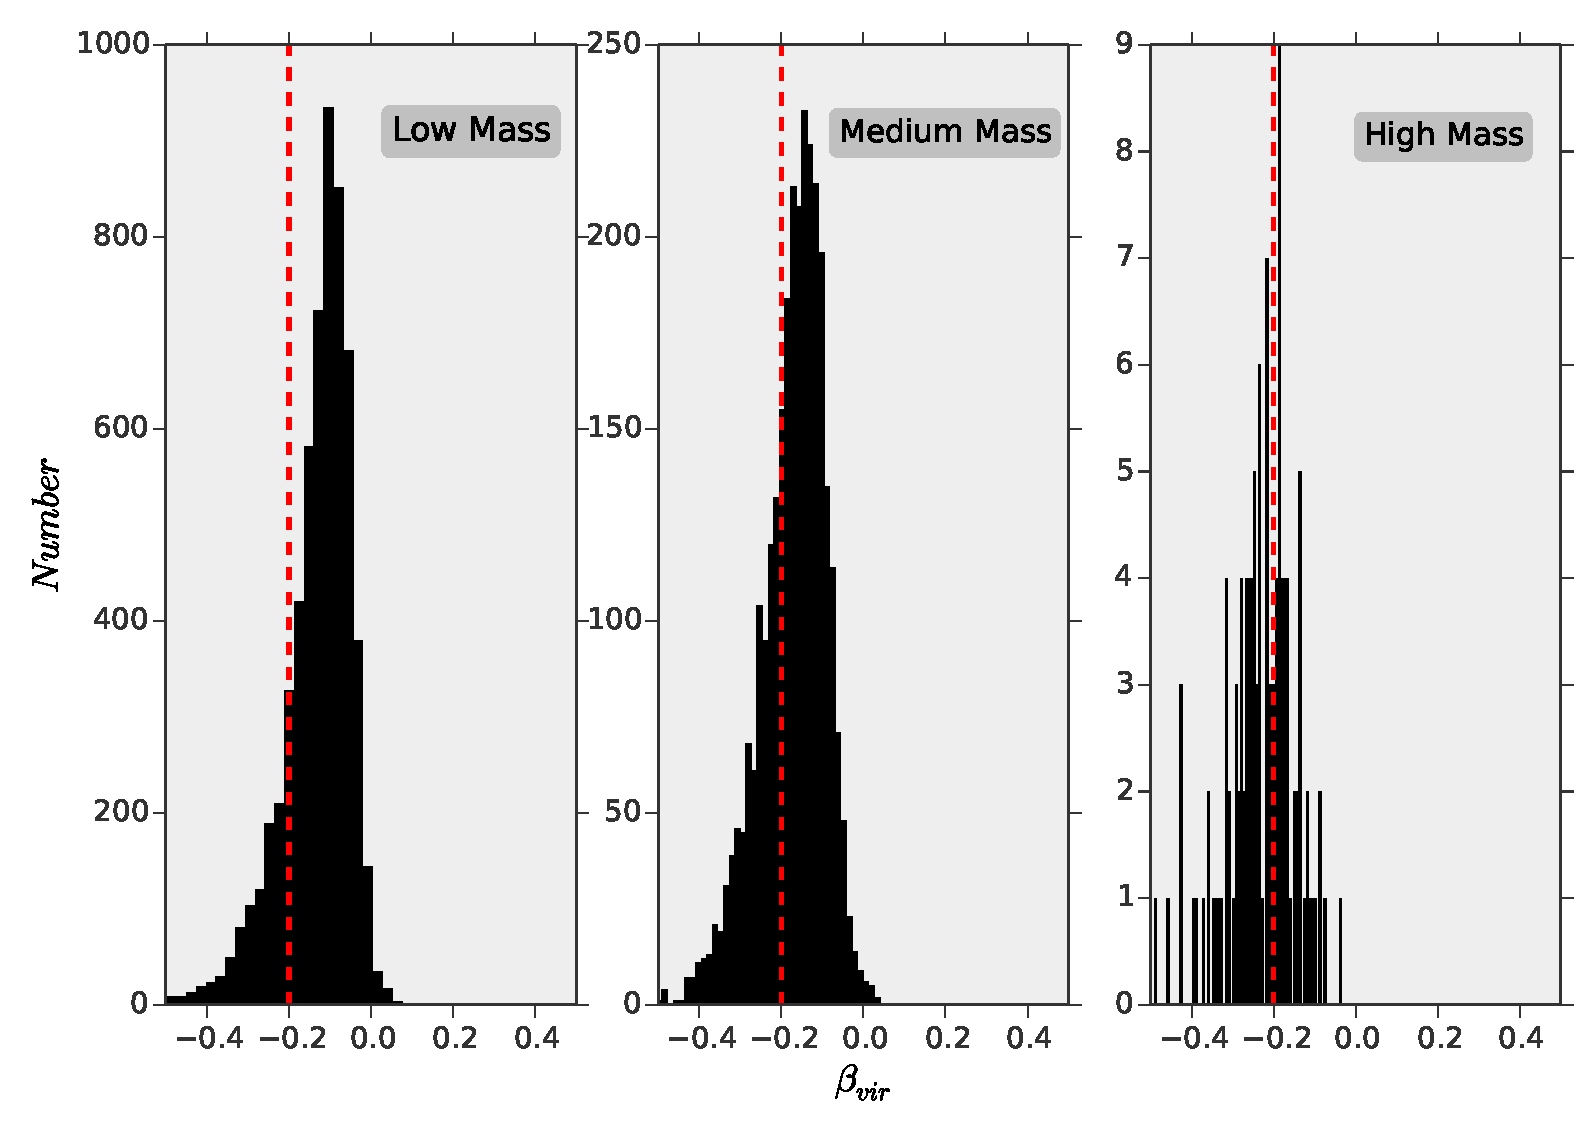
\includegraphics[width=\textwidth]{images/ClusterProjectionProject/Beta_Distributions2.eps}
\end{array}$
\end{center}
\caption[The Virial $\mathrm{\beta}$ Parameter]{The distributions of virial $\mathrm{\beta}$ parameters, for the low,
  medium, and high mass samples.}
\end{figure}

All analysis results for each cluster halo within this study have been
stored in a downloadable database\footnotemark
\footnotetext[2]{http://www.physics.drexel.edu/$\sim$groenera/zodb$\_$file.fs}. 

\section{Results}
Based upon the above criteria, that a halo must be both virialized and 
best fit by a single component halo model, we find that  $55.3\%$,
$42.0\%$, and $17.4 \%$ of halos in the low, medium, and high mass
samples make it through our selection criteria. This tendency
 of finding higher mass halos in an un-relaxed state is a natural
 prediction of hierarchical structure formation models, since the
 largest halos are the last structures to form and must undergo major
 merging events. Additionally, nearly  all of these cluster halos can be
 described as being prolate ellipsoids, becoming marginally more spherical with
 increasing distance from the cluster center (See Figure 2.5-2.7; See Table 2.2 for a
summary of these shape results).  

\begin{table}
\begin{center}
\caption{Cluster Halo Geometry}
\label{table-2}
\begin{tabular}{@{}lcccccc}
\hline
\hline
\textbf{Radial Scale}& & & & \textbf{Low} & \textbf{Medium} & \textbf{High} \\ 
\hline
$0.5 \cdot r_{200}$ & & $\bar{p} \pm \sigma_{p}$ & & $0.67 \pm 0.15$ & $0.62 \pm 0.14$ & $0.56 \pm 0.13$ \\
& & $\bar{q} \pm \sigma_{q}$ & & $0.53 \pm 0.12 $ & $0.49 \pm 0.11$ & $0.42 \pm 0.06$ \\
\hline
$r_{200}$ & & $\bar{p} \pm \sigma_{p}$ & & $0.71 \pm 0.13$ & $0.66 \pm 0.13$ & $0.54 \pm 0.15$ \\
& & $\bar{q} \pm \sigma_{q}$ & & $0.57 \pm 0.11$ & $0.52 \pm 0.10$ & $0.42 \pm 0.08$ \\
\hline
$2 \cdot r_{200}$ & & $\bar{p} \pm \sigma_{p}$ & & $0.69 \pm 0.12$ & $0.67 \pm 0.12$ & $0.54 \pm 0.12$ \\
& & $\bar{q} \pm \sigma_{q}$ & & $0.55 \pm 0.10$ & $0.53 \pm 0.10$ & $0.43 \pm 0.08 $ \\
\hline
\end{tabular}

\medskip
Reported here are the sample mean (standard deviation) values of the
semi-intermediate to semi-major axis ratio $p$, and semi-minor to semi-major
axis ratio $q$ for each mass sample (virialized, non-mergers) at various
physical scales of interest.
\end{center}
\end{table}

\begin{figure}
\begin{center}$
\begin{array}{c}
  \includegraphics[width=0.65\textwidth]{images/ClusterProjectionProject/LMSingleVirialHalf.pdf} \\
  \includegraphics[width=0.65\textwidth]{images/ClusterProjectionProject/LMSingleVirialFull.pdf}
\end{array}$
\end{center}
\caption[Low Mass Shape Results]{The distribution of isodensity shapes for the low mass halo sample at a radial scale of $\sim 0.5 r_{200}$. The green and blue shaded regions are the 1- and
  2-$\sigma$ gaussian error ellipses, and red indicates the sample mean.}
\end{figure}

\begin{figure}
\begin{center}$
\begin{array}{c}
  \includegraphics[width=0.65\textwidth]{images/ClusterProjectionProject/MMSingleVirialHalf.pdf} \\
  \includegraphics[width=0.65\textwidth]{images/ClusterProjectionProject/MMSingleVirialFull.pdf}
\end{array}$
\end{center}
\caption[Medium Mass Shape Results]{Same as Figure 2.5, but for the medium mass halo sample.}
\end{figure}

\begin{figure}
\begin{center}$
\begin{array}{c}
  \includegraphics[width=0.65\textwidth]{images/ClusterProjectionProject/HMSingleVirialHalf.pdf} \\
  \includegraphics[width=0.65\textwidth]{images/ClusterProjectionProject/HMSingleVirialFull.pdf}
\end{array}$
\end{center}
\caption[High Mass Shape Results]{Same as Figure 2.5, but for the medium mass halo sample.}
\end{figure}

Intrinsic NFW concentrations are shown in Figure 2.8 and are consistent
with those produced in previous simulations as well as previous
studies of the MultiDark simulation \citep{PradaEtAl2012}.  As expected, halo
concentrations decrease with increasing halo mass. This
concentration-mass relationship is generally fit with a power-law model which
takes the form:  
\begin{equation}
\mathrm{c_{200} = \frac{c_{0}}{\left( 1+z \right)^{\beta}} \left( \frac{\mathrm{M}_{200}}{\mathrm{M}_{*}} \right)^{\alpha}}
\end{equation}
where for our sample $\mathrm{z=0}$, and we use M$_{*}= 10^{14} \mathrm{h}^{-1}
$M$_{\odot}$ (Figure 2.9). We first compute $r_{200}$ from the
cumulative density profile of each halo, and thus establishing  
M$_{200}$. Next, by fitting NFW profiles to these density profiles we
obtain concentration parameters. For MDR1 cluster halos, we find a
concentration-mass relation of  
\begin{equation}
\mathrm{c_{200} = \left( 4.775 \pm 0.022 \right) \left( \frac{\mathrm{M}_{200}}{10^{14} \mathrm{h}^{-1}
    \mathrm{M}_{\odot}} \right)^{-0.056 \pm 0.007}}
\end{equation}

\begin{figure}
 \centering
 \includegraphics[width=0.75\textwidth]{images/ClusterProjectionProject/SingleVirialConcs.pdf}
\caption[MDR1 Intrinsic Concentration Parameters]{The distributions of intrinsic concentrations for all single virialized halos of each mass sample. From top to bottom: 1) Low Mass, 2) Medium Mass, and 3) High Mass.}
\end{figure}

From the intrinsic distributions of shape and concentration found for
each sample population, we find that solely due to line-of-sight
orientation (that is, perfectly aligned with the major axis),
analytically projected concentrations tend to be 
systematically higher by about $20\%-50\%$ for virialized, single model halos. Halos with
intrinsically low concentrations have been found to suffer from a larger
orientation bias $\sim 50\%$, whereas higher intrinsic concentrations
tend to produce an over-concentration of $\sim 20\%$, albeit with much lower
scatter. Additionally, this trend tends to flatten out with
increasing distance from the cluster center. This implies that, for a fixed 
halo concentration, inner regions of halos (those probed on or near strong
lensing scales) will bias higher than outer regions of halos (those probed
on weak lensing scales) if viewed along the major axis. This information is
most saliently captured for relaxed, low mass halos (Figure 2.10; See also
Figure 2.11 for medium mass halos, and Table 2.3 for a complete summary). 

The underlying cause for this mismatch in over-concentration between
halos with low and high intrinsic concentrations is due to the magnitude of the
change in shape as a function of radius. Low concentration halos are shown to
significantly change their shape between $\mathrm{0.5 \cdot r_{200}}$ and $\mathrm{r_{200}}$,
increasing in p and q, $81\%$ and $80\%$ of the time with median differences of
$\mathrm{\Delta p = 0.14}$ and $\mathrm{\Delta q = 0.11}$ (Figure 2.12). Halos with high intrinsic 
concentrations increase in p and q $\sim 65 \%$ of the time, however,
the median value of the difference in axial ratio drops to $\sim 0.03$.

On the extreme end, we have shown that although a systematic bias
exists, certain low concentration halos ($\mathrm{c_{200}\sim 1-3}$) with extreme
axis ratios can produce upwards of a factor of two higher in projected
concentration on a case-by-case basis. This can be seen most notably
in the low and medium mass samples at $\mathrm{r\sim 0.5 \cdot  r_{200}}$.

Additionally, we also find that concentric ellipsoidal shells are well
described as being coaxial with one another, that is to say there
is insignificant amounts of twisting of isodensity surfaces for each mass
population. Alignment becomes even better with increasing radius,
where the misalignment is a maximum at the innermost radial
value (Figures 2.13-2.15). It should be noted, however, that alignment results
are expected to be biased low due to correlation between each ellipsoidal
surface and ones interior to it. Though the aggregate shows relatively
good alignment, it is again possible for individual cluster halos to produce
significant ($\la 30^{\circ}$) offsets between projected isodensities
located at strong and weak lensing scales. This fact alone complicates
things; however, in the limit of large numbers of cluster halos, this
effect should be minimal in biasing reconstructed concentrations for
the population as a whole.  

\begin{figure}
\centering
\includegraphics[width=0.75\textwidth]{images/ClusterProjectionProject/cM_slope.pdf}
\caption[The Intrinsic MDR1 c-M Relation]{Shown here is the intrinsic concentration-mass relationship for the MDR1 cosmological simulation run. Orange stars represent values of concentration from the analytical expression found in \citet{PradaEtAl2012} at redshift $z=0$ for values of halo mass corresponding to the sample used in this study.}
\end{figure}

\section{Summary and Conclusions}

We have shown that relaxed MultiDark MDR1 simulation (FOF) cluster
halos, which are well described by a single NFW density profile, are
primarily prolate spheroidal in geometry and become increasingly more spherical with
increasing radius from the cluster center of mass. Using shape on weak
and strong lensing scales as well as derived concentrations,
we analytically project these halos along the line of sight. In doing
so, we find that low mass clusters are typically over-concentrated by
about 56\% and 20\% at half $\mathrm{r_{200}}$ for concentrations  between
1-3 and 7-10, respectively. At $\mathrm{r_{200}}$ this enhancement drops to
38\% and 19\%. What this tells us is that the average projected
concentration differs by about 18\% for halos with intrinsically low
concentrations simply due to differences in halo geometry as a 
function of radius. Clusters which do not meet this criteria show the
opposite trend in shape, becoming more prolate with increasing radius. 

Strong lensing clusters are usually identified by their hard to miss
tangential or radial arcs, and are expected to represent a biased
population simply because large mass and alignment along the line of
sight are key ingredients in producing large Einstein radii. If these
lensing clusters are in fact preferentially aligned along the line of
sight (and are relaxed), we would expect that all else being 
equal weak lensing reconstructions should under-estimate the
concentration for a population of such objects.   
  
Projection effects aside, additional complications arise in measuring
halo concentration using strong and weak lensing. For example, halo
substructure can play a significant role in altering the shape of the
lens as seen by strong lensing \citep{MeneghettiEtAl2007},  along with
massive objects unassociated with the halo which lay along the line of
sight \citep{PuchweinHilbert2009}.  \citet{RedlichEtAl2012} also find
that cluster mergers bias high the distribution of Einstein Radii,
highlighting another source of potential bias. The weak lensing signal
can be diminished by things like atmospheric PSF, correlations in the
orientation of background galaxies due to large scale structure, among
the usual sources of uncertainty in measuring galaxy shapes (for a
review of galaxy shape measurement and correlation of galaxy shapes,
see \citealt{HoekstraJain2008}; for a discussion of cluster triaxiality
and projections of large scale structure see
\citealt{BeckerKravtsov2011}). Lastly, \citet{GiocoliEtAl2014}
  conclude through simulations that the use of a generalized NFW model
  reduces mass and concentration reconstruction biases for clusters
 containing a BCG and adiabatic contraction of the dark matter. They
 also find that halo parameters differ between WL and WL+SL
 reconstruction methods, and that strong lensing selected clusters can
have concentrations 20-30\% in excess of the expected average at fixed
mass. 

\begin{table}
\begin{center}
\caption{Concentration Enhancements}
\label{table-3}
\begin{tabular}{@{}lcccccc}
\hline
\hline
\textbf{Radial Scale}& & \textbf{Low Mass} & & \textbf{Medium Mass} \\ 
& $c_{200}$ & $\bar{\Delta}_{c_{200}} \pm \sigma_{\Delta}$ & $c_{200}$ & $\bar{\Delta}_{c_{200}} \pm \sigma_{\Delta}$ \\ 
\hline
$0.5 \cdot r_{200}$ & $[1-3]$ & $1.56 \pm 0.29$ & $[1-3]$ & $1.52 \pm 0.25$\\
& $[7-10]$ & $1.20 \pm 0.07$ & $[6-9]$ & $1.26 \pm 0.09$ \\
\hline
$ r_{200}$ & $[1-3]$ & $1.38 \pm 0.16$ & $[1-3]$ & $1.43 \pm 0.15$\\
& $[7-10]$ & $1.19 \pm 0.09$ & $[6-9]$ & $1.24 \pm 0.09$\\
\hline
$1.5 \cdot r_{200}$ & $[1-3]$ & $1.30 \pm 0.12$ & $[1-3]$ & $1.34 \pm 0.11$ \\
& $[7-10]$ & $1.17 \pm 0.07$ & $[6-9]$ & $1.22 \pm 0.09$ \\
\hline
$2 \cdot r_{200}$ & $[1-3]$ & $1.28 \pm 0.11$ & $[1-3]$ & $1.31 \pm 0.10$\\
& $[7-10]$ & $1.18 \pm 0.07$ & $[6-9]$ & $1.23 \pm 0.09 $ \\
\hline

\end{tabular}

\medskip
Average Concentration Enhancement ($\mathrm{\Delta_{c_{200}} \equiv
C_{200}/c_{200}}$) on Weak and Strong Lensing Scales for Low and Medium
Mass Samples.
\end{center}
\end{table}


\begin{figure}
\begin{center}$
\begin{array}{c}
  \includegraphics[width=0.75\textwidth]{images/ClusterProjectionProject/LMSingleVirialHalfConcsLOS.pdf} \\
  \includegraphics[width=0.75\textwidth]{images/ClusterProjectionProject/LMSingleVirialFullConcsLOS.pdf}
\end{array}$
\end{center}
\caption[Low Mass Concentration Enhancements]{Shown here are concentration enhancements against intrinsic
  halo concentrations for line-of-sight oriented halos for the low
  mass, single-model, relaxed halo population.  In the top (bottom) panel,
  we show the population at $\mathrm{\sim 0.5 \cdot r_{200}}$ ($\mathrm{\sim 1 \cdot
  r_{200}}$). Overplotted are the mean and standard deviation of low
  ($\mathrm{1 \le c_{200} \le 3}$) and high ($\mathrm{7 \le c_{200} \le 10}$)
  concentration halos for comparison. We find two novel trends: 1) the
concentration enhancement is a function of the radial scale within the
halo, where inner regions are found to be significantly higher than
outer regions; this feature is most noticeable for halos with
intrinsically low concentrations,  and 2) the concentration
enhancement is a function of the intrinsic halo concentration (albeit
with some scatter).} 
\end{figure}

\begin{figure}
\begin{center}$
\begin{array}{c}
  \includegraphics[width=0.75\textwidth]{images/ClusterProjectionProject/MMSingleVirialHalfConcsLOS.png} \\
  \includegraphics[width=0.75\textwidth]{images/ClusterProjectionProject/MMSingleVirialFullConcsLOS.png}
\end{array}$
\end{center}
\caption[Medium Mass Concentration Enhancements]{The concentration enhancements against intrinsic halo concentrations
  for line-of-sight oriented halos the the medium mass, single-model, relaxed
  halo population.} 
\end{figure}

\begin{figure}
\begin{center}$
\begin{array}{cc}
  \includegraphics[width=0.5\textwidth]{images/ClusterProjectionProject/p_low_1to3_half_full.pdf} & \includegraphics[width=0.5\textwidth]{images/ClusterProjectionProject/p_low_7to10_half_full.pdf} \\
  \includegraphics[width=0.5\textwidth]{images/ClusterProjectionProject/q_low_1to3_half_full.pdf} & \includegraphics[width=0.5\textwidth]{images/ClusterProjectionProject/q_low_7to10_half_full.pdf} \\
  \includegraphics[width=0.5\textwidth]{images/ClusterProjectionProject/pq_low_1to3_half_full_diff.pdf} & \includegraphics[width=0.5\textwidth]{images/ClusterProjectionProject/pq_low_7to10_half_full_diff.pdf}
\end{array}$
\end{center}
\caption[A Summary of The Change in Shape for the Low Mass Sample]{Halos with intrinsically low concentrations exhibit a much larger change in shape as a function of radius. \textit{Upper left and middle}: Normalized distributions of axial ratios p and q for low-mass, low-concentration (1-3) halos at half $\mathrm{r_{200}}$ (blue) and $\mathrm{r_{200}}$ (green). \textit{Bottom left and middle}: The distributions of axial ratios p and q for low-mass, high-concentration (7-10) halos at half $\mathrm{r_{200}}$ and $\mathrm{r_{200}}$. \textit{Upper right, (Lower right)}: Distributions of the differences in axial ratios p (purple) and q (orange) for low-concentration (high-concentration) low-mass cluster halos.}
\end{figure}


\begin{figure}
\begin{center}$
\begin{array}{c}
  \includegraphics[width=0.9\textwidth]{images/ClusterProjectionProject/LowMass_EllipsoidAlignment_BoxViolin_Virialized.png}
\end{array}$
\end{center}
\caption[Low Mass Isodensity Alignment]{A `violin plot' for the low mass sample, showing the distribution of
  angles between the major axis of an isodensity at radial coordinate
  $\mathrm{r_{i}}$, and one at $\mathrm{r_{i} + \Delta r}$. Green shaded regions
represent the distributions of angles, and overplotted is a box plot showing
the location of the quartiles (25\%, 50\%, and 75\%).}
\end{figure}

\begin{figure}
\begin{center}$
\begin{array}{c}
  \includegraphics[width=0.9\textwidth]{images/ClusterProjectionProject/MediumMass_EllipsoidAlignment_BoxViolin_Virialized.png}
\end{array}$
\end{center}
\caption[Medium Mass Isodensity Alignment]{A `violin plot' for the medium mass sample.}
\end{figure}

\begin{figure}
\begin{center}$
\begin{array}{c}
  \includegraphics[width=0.9\textwidth]{images/ClusterProjectionProject/HighMass_EllipsoidAlignment_BoxViolin_Virialized.png}
\end{array}$
\end{center}
\caption[High Mass Isodensity Alignment]{A `violin plot' for the high mass sample.}
\end{figure}

\section{Future Work}

An explicit prediction has been made regarding the discrepancy between
projected halo concentrations of cluster halos on characteristic
lensing scales. A natural next step would be to simulate the signal
produced from gravitational lensing by conducting mock weak and strong
lensing analyses. However, one would realistically need to include the
effects of baryons. Additionally, we plan to summarize the current
state of the field of galaxy cluster mass reconstructions in each of
the methods used. In future work, we will aggregate all measured NFW
mass/concentration pairs from these methods in order to shed light on
potential systematic observational biases, particularly on strong and
weak lensing scales.  

It has yet to be determined if this effect manifests itself in a
measurable way for the cluster halo population. Follow-up observations
of strong lensing clusters could be proposed as a way of testing the
veracity of this prediction. Knowing the intrinsic distribution of
cluster concentrations is difficult if not impossible due to the
degenerate nature of the reverse-projection process. However, the shape
of the distribution of measured concentrations due to lensing could
possibly contain hallmark characteristics which could indicate the
level of line of sight biasing of the population. With this
information known, ultimately a correction procedure could then be
proposed.
  
  %CHAPTER: Observational Concentration Mass Relation
  \chapter[The Observed c-M Relation]{The Galaxy Cluster Concentration-Mass Scaling Relation}

\section{Introduction}

Galaxy clusters have long been used as probes of cosmology. Cluster
observables, like X-ray luminosity, $\mathrm{L_{X}}$, optical
richness, and line-of-sight galaxy dispersion,
$\mathrm{\sigma_{v}}$, are closely tied to the formation and evolution of
large scale structures, and scale with redshift and the mass of the
host halo \citep{SE15.3}. Scaling relations of clusters also provide a way of testing
cosmology \citep{VI09.2,RO10.1,MA10.1,MA14.1}, though are imperfect
proxies for mass, due to the 2-Dimensional view they provide for us. Large
cosmological simulations provide a detailed 3-dimensional 
view of the hierarchical process of structure formation, one that is
unattainable by even the most accurate reconstruction techniques available.

The radial density profiles of clusters, well-modeled by the universal NFW
profile (\citealt{NA97.1}; Eq. 1.1), appears to be a prevailing outcome of simulations
regardless of cosmology \citep{NA97.1,CR97.1,KR97.1,BU01.1}. However, the
details of the relationship between the two model parameters, halo mass, M, and
concentration, $\mathrm{c}$, is sensitive to small changes in initial
parameters \citep{MA08.1,CO15.1}.

Tensions exist between cluster concentrations derived from
simulations and observational measurements (see section 1.3),
have been found to differ the most for gravitational lensing techniques
\citep{CO07.1,BR08.1,OG09.1,UM11.2}. This over-concentration of clusters (in
favor of observational measurements) can be partially explained by the orientation of
triaxial structure along our line-of-sight \citep{OG05.1,SE11.1}, which has the
effect of enhancing the lensing properties \citep{HE07.1}. Neglecting halo
triaxiality \citep{CO09.1} and substructure \citep{ME10.2,GI12.1} also each
have significant effects on halo parameters. For its effect on WL and X-ray
mass estimates, see \citet{SE14.2}.

Discrepancies in how measurements of the intrinsic concentration
are made using simulations also exist, along with studies who disagree
on the inner slope of the density profile
\citep{MO99.2,GH00.1,NA04.1}. However, the most puzzling and potentially
interesting disparity between simulations is the existence of the upturn
feature in the c-M relation (see for example, Fig. 12 of \citealt{PR12.1}) at high redshift
\citep{PR12.1,DU14.1,KL14.1,DI15.1}, which some argue is an artifact caused by
the selection of halos which are dynamically unrelaxed \citep{LU12.1}. This
novel feature only shows up when the concentration is expressed as a
profile-independent halo property (in terms of the ratio of the maximum 
circular velocity and the virial velocity, $\mathrm{V_{max}/V_{vir}}$). In
terms of the classical definition of concentration, this feature disappears
(see \citealt{ME13.1}). 

The connection between the observed concentration, $\mathrm{c_{2D}}$,
and the intrinsic concentration, $\mathrm{c_{3D}}$, is further complicated,
since it has been shown that relaxed cluster isodensities are not constant
on all scales \citep{FR88.1,CO96.1,DU91.1,WA92.1,JI02.1,HA07.1,GR14.1}. Indeed,
in a previous study by \citet{GR14.1} (Chapter 2), it has been shown that a halo's concentration
is an ill-defined 2-dimensional quantity, without first specifying the scale on which the
measurement was made. Using the MultiDark MDR1 Cosmological
Simulation, \citet{GR14.1} found a systematic shift of about $\mathrm{\sim 18 \%}$ in the
mean value of the projected concentration, $\mathrm{c_{2D}}$, between weak and
strong lensing scales, for low-mass cluster halos ($\mathrm{2.5-2.6 \times
  10^{13} h^{-1} M_{\odot}}$) observed with their major axes aligned with the
line-of-sight direction. Though this difference is notably smaller than the intrinsic
scatter of the concentration parameter ($\mathrm{c_{3D}}$) for a given halo
mass, the origin of this systematic effect is solely due to the changing shape
of cluster isodensities as a function of radius.


For many objects, not only do observed concentrations seem to differ
substantially from those obtained in cosmological simulations, but
concentrations can also vary depending on which method is used. Since different
reconstruction methods probe varying scales within the halo, it is 
not unreasonable to suspect that there exist systematic differences in the
observed c-M relation caused by shape.

\bigskip

\noindent In this chapter, we focus on three main objectives.

\begin{enumerate}
\item We present the current state of the observational concentration-mass
  relation for galaxy clusters by aggregating all known measurements from the
  literature. The raw data are reported in Table A-1, and have been made
  publicly available (see Appendix A). We also provide an additional table
  (available only online), where data have been normalized over differences in
  assumed cosmology, overdensity convention, and uncertainty type found in the
  original studies.

\item We model the observed concentration-mass relation for each method,
  and compare these to one another, highlighting potential differences which
  exist, caused by the projection of structure along the
  line-of-sight, the varying shape of cluster isodensities, and the selection
  of clusters from the cosmic population.

\item Using the largest cluster sample to date, we determine
  if the observed c-M relation is consistent with theory, when
  taking halo triaxiality and elongation of structure along the line-of-sight
  into account.
\end{enumerate}

In section 3.2, we summarize many of the most common mass reconstruction
techniques which are used throughout the cluster community, and include a
discussion regarding physical scales probed within the cluster using these
methods. In section 3.3, we discuss the procedure for collecting our sample from
the literature, and normalizing over convention, cosmology, and
uncertainties. In section 3.4, we present results for the observed c-M relation
for each method, and in section 3.5, we discuss the projection of triaxial halos
from simulations to the observed lensing relations. Lastly, in section 3.6, we
conclude and discuss our findings.

Throughout this chapter we adopt a flat $\Lambda$CDM cosmology, $\Omega_{m}=0.3$,
$\Omega_{\Lambda}=0.7$, and $\mathrm{H}_{0} = 70$ $\mathrm{km}$
${\mathrm{s}}^{-1} {\mathrm{Mpc}}^{-1}$. Generally speaking, we reserve the
following colors within plots to represent the various methods: 
\begin{itemize}
\item Caustic Method (CM): blue
\item Line-of-sight velocity dispersion (LOSVD): orange
\item X-ray: green
\item Weak Lensing (WL): purple
\item Strong Lensing (SL): red
\item Weak + Strong Lensing (WL+SL): black
\end{itemize}
Unless otherwise stated, throughout the study, uncertainties are reported as
1-$\mathrm{\sigma}$ (68.3\%) Gaussian uncertainties.

\section[Reconstruction Techniques]{Cluster Mass Reconstruction Techniques}
In this section, we present a brief overview of common mass reconstruction
techniques and modeling of the cluster density profile.
\subsection{Weak Lensing (WL)}
Weak gravitational lensing is the process by which images of background galaxies
are distorted by massive foreground objects. Though these distortions cannot be
detected for any given source, it is possible to obtain a signal by
locally averaging the shapes (ellipticities) of galaxies. This shear measurement within a given
bin can be used as a direct proxy for the lens density profile at intermediate to large radii.


For a symmetric distribution, the azimuthally averaged tangential shear,
$\mathrm{\langle \gamma_{t} \rangle}$, as a function of radius from the cluster
center can then be calculated, and relates to the convergence, $\kappa$:
\begin{equation}
\mathrm{\langle \gamma_{t} \rangle (r) = \frac{\bar{\Sigma}(<r) -
    \bar{\Sigma}(r)}{\Sigma_{cr}} = \bar{\kappa}(<r) - \bar{\kappa}(r) }
\end{equation}
where the critical surface mass density is defined in terms of
cosmology-dependent angular diameter distances $\mathrm{D_{s}}$ (source),
$\mathrm{D_{ds}}$ (lens to source), and $\mathrm{D_{d}}$ (lens): 
\begin{equation}
\mathrm{\Sigma_{cr} = \frac{c^{2} D_{s}}{4\pi G D_{ds} D_{d}}}
\end{equation}
Expressions, specifically for the NFW profile, for the convergence
\citep{BA96.1} and the tangential shear \citep{WR99.1} have been
derived, and can be used for model fitting.

Weak lensing comes with its own intrinsic biases in that more massive clusters
produce larger distortions of background galaxies. As a result, in a survey of
detected clusters, the expectation is that nearly all of the most massive
clusters would be {\em selected} from the population. However, in the low mass
region, clusters which are highly triaxial and elongated along the line-of-sight (i.e. -
larger 2D concentrations) are more likely to pass the observational
signal-to-noise threshold than ones which are not. The net effect here is an
artificial steepening of the c-M relation due to selection. Furthermore,
lensing geometry plays an additional role in how clusters are
selected. Clusters which are too distant lack the requisite number 
density of background galaxies to obtain high signal-to-noise
\citep{BA01.1}. Table 3.1 presents the range in redshift for weak lensing
clusters, where most measurements are found to lie in the redshift range of
$\mathrm{z=0.2-0.6}$, with $\mathrm{M_{vir} \gtrsim 1\times 10^{14}
  M_{\odot}}$.

\subsection{Strong Lensing (SL)}
A natural extreme of the phenomenon of gravitational lensing can occur
if a background galaxy is serendipitously aligned with the core of
a cluster. In such cases, the projected surface mass density is so high that
multiple images of the object are produced, commonly distorting them so much
that they appear arc-like.

A density profile can be obtained by fitting a model to the observed image
positions, orientations, and fluxes, though this technique
constrains the cluster profile on small scales (approximately the Einstein radius,
$\mathrm{ \theta_{E}}$\footnote[1]{The Einstein radius for a point mass is
  $\mathrm{\theta_{E} = \left( \frac{4GM}{c^{2}} \frac{D_{LS}}{D_{L}D_{S}}
    \right)^{1/2}}$. Though there is no corresponding functional form for an
  NFW profile,  typical values for clusters lie in the range: 10''-45''
  \citep{KN03.1,BR05.2}.}, which is typically $\mathrm{\sim 5\%}$ of the virial
radius, $\mathrm{r_{vir}}$, or $\mathrm{\sim 50\%}$ of the scale radius,
$\mathrm{r_{s}}$ \citep{OG09.2}).

Due to the irregular occurrence of multiple images and arcs, cluster
measurements made with strong lensing are particularly prone to selection
effects, and likely represent a biased sampling of the cosmic
population. In fact, the efficiency of lensing is increased with increasing
mass and concentration, and a preferential line-of-sight alignment of the
triaxial halo \citep{OG09.2}. Concentrations derived from this method have been
contentiously high as compared to X-ray studies \citep{CO07.1}.

\subsection{Weak+Strong Lensing (WL+SL)}
Combining weak and strong gravitational methods constrains the density
profile over a wide range of scales, and also has the ability to break the
mass-sheet degeneracy \citep{SC95.1}. Recent efforts to combine these methods
have become more prevalent in the literature (\citet{ME14.1} - 
CLASH; \citet{OG12.1} - SGAS), and work to reconstruct the lensing potential by
minimizing a combined least-squares approach. 
\begin{equation}
\mathrm{\phantom{.} \chi^{2}(\psi) = \chi^{2}_{w}(\psi) + \chi^{2}_{s}(\psi)}.
\end{equation}


\subsection{X-ray}
Massive clusters are significant sources of X-ray radiation, due to the hot
diffuse plasma ($\mathrm{k_{B}T_{e} \sim 10 \, keV}$) emitting via thermal
bremsstrahlung, and can be used to determine the total distribution of
mass. Under assumptions of spherical symmetry and hydrostatic equilibrium with
the underlying potential \citep{EV96.1}, temperature and gas density
information, $\mathrm{\rho_{g}}$, are used to determine the total mass of the
cluster, typically at intermediate scales ($\mathrm{\sim r_{500} }$,
corresponding to the radius at which the average density inside is 500 times
$\mathrm{\rho_{cr}}$).
\begin{equation}
\mathrm{M(r) = \frac{k T(r)}{G\mu m_{p}} r \left( \frac{d \log \rho_{g}(r)}{d \log
  r} + \frac{d \log T(r)}{d \log r} \right) }
\end{equation}

These assumptions are often violated due to non-thermal pressure sources,
temperature inhomogeneity, and to the presence of substructures further out
\citep{RA12.1}, and bias low mass estimates by 25-35\%.

\subsection{Line-of-sight Velocity Dispersion (LOSVD)}
The distribution of mass within clusters can also be obtained by using the
kinematics of cluster galaxies, specifically, by using the moments of
the velocity distribution. Reconstruction methods, developed by
\citet{LO02.1} and \citet{LO03.1}, use the second (dispersion) and fourth
(kurtosis) moments of the velocity distribution, which
relies on the  underlying gravitational potential. Assuming the distribution of
mass follows an NFW profile, free parameters, which include $\mathrm{M_{vir}}$
and $\mathrm{c_{vir}}$, can be fit to the observed data.

The business of identifying clusters as mass over-densities, determining
cluster membership, removal of interlopers, and reconstruction details vary from
technique to technique. For a more complete review of the reconstruction
methods and their impact on cluster observables, see \citet{OL14.1}.

\subsection{The Caustic Method (CM)}
With the exception of weak lensing, the caustic method is the only other
standalone method which has been successful in probing the density profile at
large distances from the cluster center ($\mathrm{\gtrsim r_{vir}}$). Cluster
galaxies, when plotted in line-of-sight velocity versus projected
cluster-centric distance phase-space, create a characteristic ``trumpet
shape'', the boundaries of which form what is referred to as caustics
\citep{KA87.1,RE89.1}. The existence of these caustics mark an important
boundary which envelops a volume of space in which galaxies are gravitationally
bound to the cluster. Outside of this turnaround radius, galaxies are
ultimately carried away in the Hubble flow.

The width of the caustic (velocity) at any given projected radius,
$\mathcal{A}\mathrm{(R)}$, can then be related to the escape velocity due to
the gravitational potential of the cluster, under the assumption of spherical
symmetry \citep{DI97.1}. Through simulations of structure formation,
\citet{DI99.1} has shown that the caustic amplitude can be related to the mass
interior to radius $\mathrm{r}$ by: 
\begin{equation}
\mathrm{GM(<r) = \frac{1}{2} \int_{0}^{r} \mathcal{A}^{2}(R) \, dR }.
\end{equation}

The success of the caustic method is independent of any assumptions regarding
dynamical equilibrium of the cluster, and has been used to reconstruct profiles
over a larger range of scales: from the inner regions to a few times the virial
radius (CAIRNS: \citealt{RI03.1}; CIRS: \citealt{RI06.1}; HeCS:
\citealt{RI13.1}). However, this technique requires the measurements of at
least 30-50 cluster members, and thus limits this method to clusters at relatively low
redshifts compared to lensing and X-ray techniques. More recently,
\citet{RI13.1} make use of this technique using $\mathrm{\sim 200}$ cluster
members.

\subsection{Hybrid Techniques}
The aforementioned methods represent the most commonly applied techniques for
constructing a density profile, however, they do not represent them all. Novel
combinations of methods have also been used, but could not be included in a
study of this kind. For instance, \citet{LE08.1} combine joint lensing and
X-ray methods to make a determination of Abell 1689. \citet{TH10.1} and
\citet{VE11.1} use a combination of lensing and dynamics. Additionally, In an
attempt to only compare methods used in \citet{CO07.1}, we consciously
leave out measurements made with the Sunyaev-Zel'dovich (SZ) effect, or which use
combinations of techniques one of which uses SZ.

Previous studies have even employed these multi-technique reconstructions to
clusters in an attempt to break the line-of-sight mass degeneracy (for a review
of these techniques, see section 2 of \citet{LI13.1}; see also \citet{AM07.1},
\citet{SE12.1}). However, it is unclear if techniques such as this can adapt to 
arbitrarily complicated profiles, where shape is scale-dependent, or where
isodensities are not co-axial with one another (isodensity twisting).

\section{The Sample}

The sample of clusters collected from the literature consists of a
total of 781 cluster measurements, reported by 81 studies (Table A-2), representing the
largest known collection of cluster concentration measurements to date. Of
these, there are 361 unique clusters, giving us a sizable sampling of
the cluster population as a whole, in addition to multiple measurements of
individual clusters (often coming from more than one category of
reconstruction technique).

This study builds off of work done by \citet{CO07.1}, which aggregated 182
cluster measurements of 100 unique cluster objects. In accordance with that
study, we also report measurements of concentration (and mass) in the most
popular conventions, $c_{200}$, and $c_{vir}$. 

Table 3.1 presents population averages of masses and concentration, as well as
their range in redshift for the six reconstruction techniques we reference
throughout this study. This information highlights the importance of the
selection function of clusters, though we make no attempt in this chapter to
distinguish between whether a lack of measurements of certain values for a given
method is due to its inability to make these determinations, or whether it is
simply a preferential selection effect. In Figure 3.1, we show the
locations of galaxy clusters on the sky, as well as distributions in
mass-redshift space for each method.

\setcounter{table}{0}
\begin{landscape}
\begin{table}
caption{Population Overview}
\label{tab1}
\begin{tabular}{@{}lllcccllllll}
\hline
\hline
 Method &$\mathrm{N_{meas}}$&$\mathrm{N_{cl}}$&$\mathrm{min(M_{vir})}$
              &$\mathrm{\langle M_{vir} \rangle}$ 
 &$\mathrm{max(M_{vir})}$ &$\mathrm{min(c_{vir})}$&$\mathrm{\langle c_{vir} \rangle}$ 
 &$\mathrm{max(c_{vir})}$& $\mathrm{min(z)}$ & $\mathrm{\langle z
                                                     \rangle}$
                            &$\mathrm{max(z)}$\\ 
&&&$\mathrm{(10^{14}M_{\odot})}$&$\mathrm{(10^{14}M_{\odot})}$&$\mathrm{(10^{14}M_{\odot})}$&&&&&&\\
\hline
CM & 82 & 79 & $<$1.0 & 3.9 & 18.6 & $<$2.0& 8.9 &36.7 & 0.003& 0.06&0.44\\
LOSVD & 70 & 59 & 1.3& 5.8 & 17.1& $<$2.0& 8.8& 39.0& 0.01& 0.06&0.44\\
X-ray & 290& 195 & $<$1.0 & 26.1 & $>$40.0& $<$2.0& 7.2& 26.2& 0.003 & 0.22&1.41\\
WL & 169 & 111 & $<$1.0 & 12.4 & $>$40.0& $<$2.0& 8.1& 64.5& 0.02& 0.48 &1.45 \\
WL+SL & 113 & 58 & $<$1.0 & 8.7 & 31.8 & 2.3& 10.2& 30.6& 0.18& 0.53 &1.39\\
SL & 19 & 11 & 3.2& 24.3 & $>$40.0 & 3.8& 11.2& 27.5& 0.18& 0.47 &0.78\\
\hline
\hline
\end{tabular}
\end{table}
\end{landscape}

\begin{figure}
\begin{center}
\includegraphics[width=\textwidth]{./images/CMRelationProject/PopulationOverview1.pdf}
\end{center}
\caption[Cluster Population Overview]{(Left) The distribution of clusters on the sky for each reconstruction
  method. The dotted line shows the location of the plane of the Milky Way
  galaxy. (Right) The range of redshift and cluster masses each method spans
  for the sample we have collected.}
\end{figure}


\subsection{Normalization Procedure}

Due to the nature of this study, cluster measurements must be properly
normalized to ensure that they are compared to one another on equal footing. In
this section, we discuss the steps taken to eliminate biases due to overdensity
convention, assumed cosmology, and due to differences in the definitions of
measurement uncertainty, respectively. 

\centerline{{\large Convention}}
Under the assumption that the radial density profile follows an NFW profile,
\citet{HK03.1} derive a procedure for the conversion of both concentration and
mass between any two arbitrary characteristic radii. We apply these 
formulae as a first round of our normalization procedure.
\centerline{{\large Cosmology}}
Measurements taken from the literature do not always use the same
fiducial cosmology, and thus are not immediately comparable. Because of this,
we develop a procedure for converting measurements between any two arbitrary
cosmologies. Appendix B outlines this procedure for general lensing methods.

For extreme cosmologies, the correction to the concentration parameter,
$\mathrm{c_{vir}}$, and mass, $\mathrm{M_{vir}}$, are approximately 5$\%$ and
10$\%$, respectively. This correction is significantly smaller than other known
effects. Moreover, the vast majority of all measurements we have collected
assume flat cosmologies which lie in the range $\mathrm{\Omega_{\Lambda} = 1 -
  \Omega_{m}  = 0.73 - 0.68}$. The corrections to the concentration and mass in
this range are $\mathrm{\sim 1\%}$. Figure 3.2 shows the fractional error in
concentration and mass, over the full range of flat cosmologies. 

\begin{figure}
\begin{center}
\includegraphics[width=\linewidth]{./images/CMRelationProject/CosmoCorrection.png}
\end{center}
\caption[Concentration/Mass Cosmology Correction]{The fractional error in weak lensing concentration and mass
  measurements due to the conversion to an arbitrary cosmology (x-axis) from the
  fiducial cosmology used in this chapter.}
\end{figure}


\centerline{{\large Uncertainties}}
Another complication which must be accounted for is the usage of
multiple definitions of measurement uncertainty on resulting mass
and concentration estimates reported throughout the literature. Particularly,
many fitting procedures (namely methods which involve brute force exploration
of likelihood space) produce maximum-likelihood estimates of
parameters of interest and corresponding confidence intervals. However, most
studies do not report the marginal distributions from their fitting procedures,
and consequently, limits the utility of their measurements for those looking to
compare or adopt their values.

Furthermore, the mathematical theorems which dictate the propagation
of error of measurements rely on expected values and variances, rather
than maximum-likelihood estimates and probability
intervals. \citet{DA04.1} argues that the expected value and standard
deviation should {\em always} be reported, and in the event of an
asymmetric distribution, one should also report shape parameters or
best-fit model parameters as well. Most importantly, any published
result containing asymmetric uncertainties causes the value of the
physical quantity of interest to be biased.

We follow the procedure outlined in \citet{DA04.1} for symmetrizing
measurements with asymmetric uncertainties (to first order),
$\mathrm{{\theta_{m}}^{\Delta_{+}}_{\Delta_{-}}}$, and apply this to both
cluster mass and concentration measurements.

\begin{subequations}
\begin{align}
\mathrm{\sigma_{\theta} \approx \frac{\Delta_{+} + \Delta_{-}}{2}}\\
\mathrm{E[\theta] \approx \theta_{m} + \mathcal{O}(\Delta_{+} - \Delta_{-})}
\end{align}
\end{subequations}

Additionally, many studies report measurements without uncertainties
altogether. For these clusters, we apply uncertainty based upon the
estimate of the average fractional uncertainty of all other
measurements of its type. The most notable method having this issue is
the caustic method, where virtually no measurements are accompanied by
uncertainties. In this case, we apply the same fractional uncertainty
to all measurements equally, and is derived from the average fractional error
of LOSVD concentration and mass measurements.

Lastly, a large fraction of clusters represented in our database have multiple
concentration and mass measurements, leading subsequent fits to be more
sensitive to these particular objects. In order to prevent fits from being
dominated by the most popular clusters (e.g. - Abell 1689, of which there are
26 measurements in total), we combine similar measurements using an
uncertainty-weighted average value.

\section[The Observed c-M Relation]{The Observed Concentration-Mass Relation}

In Figure 3.3, we show the full cluster dataset after applying the normalization
procedures discussed in the previous section. Following this,
we present here the results of our fitting procedure to these data. The typical
prescription for modeling the c-M relation, is to use a double power-law model
of the following form
\begin{equation}
\mathrm{c(M) = \frac{A}{\left(1+z\right)^{\beta}} \left(\frac{M}{M_{*}}\right)^{\alpha}}
\end{equation}
where the power-law indices, $\mathrm{\alpha}$ and $\mathrm{\beta}$, control
the dependence of the concentration with respect to mass and redshift. The
model parameter, $\mathrm{A}$, controls the normalization of the relation, once a
suitable $\mathrm{M_{*}}$ has been chosen ($\mathrm{M_{*}=1.3\times10^{13}
  h^{-1} M_{\odot} = 1.857\times 10^{13} M_{\odot}}$). 

\begin{figure}
\begin{center}
\includegraphics[width=\textwidth]{./images/CMRelationProject/CMRelation_FullSample_Symmetrized.png}
\end{center}
\caption[The Normalized Data]{The full normalized observational cluster sample, colored by
  method. Uncertainties have been omitted here for clarity.}
\end{figure}


We follow convention in using the above model, but in a slightly different
form, with the power-law index, $\beta$, fixed to unity. We adapt this model to
a linear model in the following way
\begin{equation}
\mathrm{\mathcal{Y} = m\mathcal{X}+b \pm \sigma_{int}}
\end{equation}
where variables and model parameters relate to the initial model in the
following way:
\begin{subequations}
\begin{align}
\mathrm{\mathcal{Y}}&\mathrm{\equiv \log c (1+z)}\\
\mathrm{\mathcal{X}}&\mathrm{\equiv \log M}\\
\mathrm{m}&\mathrm{= \alpha}\\
\mathrm{b}&\mathrm{= \log A - \alpha \log M_{*}}
\end{align}
\end{subequations}

We introduce the intrinsic scatter, $\mathrm{\sigma_{int}}$, as a fixed parameter,
which we estimate from the data (independently from the fit
itself), and is assumed to be constant over the full mass range:
\begin{equation}
\mathrm{\sigma_{int}^{2} = \sigma_{res}^{2} - \langle \sigma_{\mathcal{Y}}^{2} \rangle}
\end{equation}
where $\mathrm{\sigma_{res}}$ is the scatter in the residual between the data and the
best-fit model, and $\mathrm{\langle \sigma_{\mathcal{Y}}^{2} \rangle}$ is the
average squared-uncertainty in the dependent variable. The idea here is that the
scatter in the residual must be accounted for by a combination of scatter due
to the intrinsic relation itself as well as the uncertainties in the
measurements of the observables. We also note that although the value of the
redshift for any given cluster has an effect on the uncertainty of the variable
$\mathrm{\mathcal{Y}}$, the uncertainty in the measured redshifts themselves do
not contribute much to the overall uncertainty of the best-fit model parameters.
 
After measurements have been normalized, we eliminate extreme values of mass
and concentration. Simulations tell us that the most massive clusters which
exist at present are approximately a few times $\mathrm{10^{15} \,
  M_{\odot}}$. Accordingly, we remove masses which are larger than
$\mathrm{4\times 10^{15}\,M_{\odot}}$. We also remove masses lower than
$\mathrm{1\times 10^{14}\, M_{\odot}}$, as these are more typical masses of
groups. Lastly, concentrations which are lower than 2, indicate rather poor NFW
fits to the density profile, and will bias our inferred parameters.

In Table 3.2, we present our best-fit linear model parameters, and their mapping
back to the original power-law model. In Figure 3.4, individual fits
to each subsample are shown alongside normalized data points. Lensing (WL
and WL+SL) and X-ray relations show a clear trend consistent with concentration
decreasing with increasing mass. We also include a bootstrap analysis of
these fits, to reveal the sensitivity of the fits to the data. 

Though seemingly well-constrained, the bootstrap analysis reveals that our
strong lensing c-M relation is highly sensitive to the dataset (due to the very
small sample size), and so the best-fit model parameters are likely
untrustworthy.

General agreement between concentration and mass measurements of all methods
can be seen in the range $\mathrm{10^{14.5}-10^{15} M_{\odot}}$, which we also point
out, is the region we find most consistent with simulation results.

%\setcounter{table}{0}
\begin{landscape}
\begin{table}
\begin{minipage}{210mm}
\caption{Best-Fit Concentration-Mass Relation Parameters}
\label{tab2}
\begin{tabular}{@{}llllllllllllllll}
\hline
\hline
 Method & & & & & & & & & & \multicolumn{3}{l}{Bootstrap $\rightarrow$}& & & \\ 
\hline
 &$\mathrm{N_{cl}}$&$\mathrm{m}$\footnote[1]{The slope, $\mathrm{m}$, of the
 linear model is exactly equivalent to the power-law index
 $\mathrm{\alpha}$.}&$\mathrm{\sigma_{m}}$\footnote[2]{$\mathrm{\sigma_{m} =
                      \sigma_{\alpha}}$} &$\mathrm{b}$ 
                &$\mathrm{\sigma_{b}}$ &$\mathrm{A}$\footnote[3]{The
                                         normalization parameter, $\mathrm{A}$,
                                         depends upon both $\mathrm{m}$ and $\mathrm{b}$:
                                         $\mathrm{A=10^{b+m\log M_{*}}}$}
                    &$\mathrm{\sigma_{A}}$\footnote[4]{Uncertainty was
                      propagated through the expression in [3].}
                    &$\mathrm{\sigma_{int}}$\footnote[5]{Equivalent to the
                      scatter in $\mathrm{\log c_{vir}}$ reported in previous studies.}& $\mathrm{\chi^{2}_{red}}$& $\mathrm{m}$ &$\mathrm{\sigma_{m}}$ &$\mathrm{b}$
                            &$\mathrm{\sigma_{b}}$ &$\mathrm{A}$
                                                          &$\mathrm{\sigma_{A}}$\\
\hline
CM & 63 & 0.280 & 0.003 & -3.138 & 0.038 & 3.778 & 0.677 & 0.242 & 0.327 & 0.28& 0.19& -3.16&2.73 & 3.59&43.43\\
LOSVD & 58 & 0.010 & 0.002 & 0.728& 0.025 & 7.256 & 0.861 & 0.228 & 1.000 & 0.13& 0.17& -1.00& 2.55& 5.31&58.74\\
X-ray & 149 & -0.105 & 0.001 & 2.494 & 0.010 & 12.612 & 0.676 & 0.160 & 1.224 &-0.17 & 0.03& 3.38& 0.44& 13.32&25.69\\
WL & 93 & -0.379 & 0.001 & 6.576 & 0.014 & 35.246 & 2.213& 0.118 & 1.302 & -0.43& 0.11& 7.35& 1.62& 44.10&312.68\\
WL+SL & 57 & -0.534 & 0.001 & 8.977& 0.016 & 77.882 & 5.249 & 0.130 & 1.070 & -0.54& 0.10& 9.10& 1.46& 86.06&552.28\\
SL & 10 & 0.097 & 0.004 & -0.422 & 0.062 & 7.236 & 1.951 & 0.254 & 1.003 & 0.11& 0.23& -0.60& 3.49& 7.24&109.02\\
\hline
All (This Work) & 293 & -0.152 & 0.001 & 3.195 & 0.007 & 15.071 & 0.703 & 0.146 & 1.354 & -0.16& 0.03& 3.26& 0.44& 13.71&26.45\\
All (CO07.1)& 62 & -0.14 & 0.12 & -- & -- & 14.8 & 6.1 & 0.15 & -- & -- & -- & -- & -- & -- & --\\
\hline
\hline
\end{tabular}
\end{minipage}
\end{table}
\end{landscape}

\begin{figure}[h!]
\begin{center}
\includegraphics[width=\textwidth]{./images/CMRelationProject/FitToEachMethod.png}
\end{center}
\caption[Observed c-M Fits]{Upper left to lower right: Individual fits to CM, LOSVD, X-ray,
    WL, WL+SL, and SL. The shaded regions represent the 1-$\mathrm{\sigma}$ uncertainty
    in the best-fit parameters, and includes the intrinsic scatter, $\mathrm{\sigma_{int}}$. These
    relations are extrapolated over the full range of cluster masses for
    illustration purposes only. }
\end{figure}

We also compare our results to the c-M relation studied by CLASH, which use
a combined weak and strong lensing technique for 19 X-ray selected galaxy
clusters. The relation they fit,
\begin{equation}
\mathrm{c_{200} = A \left( \frac{1.37}{1+z} \right)^{B} \left(
    \frac{M_{200}}{8\times 10^{14} h^{-1} M_{\odot}} \right)^{C}}
\end{equation}
with best-fit values of $\mathrm{A=3.66\pm0.16}$, $\mathrm{B = -0.14\pm0.52}$,
and $\mathrm{-0.32\pm0.18}$, agrees well with projected simulations, after
accounting for the X-ray selection function. Figure 3.5 shows the comparison of
the CLASH c-M relation to the the lensing relations, WL and WL+SL. Our
relations are significantly steeper, and have higher
normalizations\footnote[2]{Due to the addition of a third model parameter, the 
  CLASH normalization is not directly comparable to ours. However, visual
  inspection of Fig. 3.5 shows that their value is certainly lower than ours.},
though it should be noted that we do not account for the lensing selection
function, which we would expect to lower both parameters.

\begin{figure}
\begin{center}$
\begin{array}{cc}
\includegraphics[width=0.5\textwidth]{./images/CMRelationProject/Clash_Comparison_02.png} &
  \includegraphics[width=0.5\textwidth]{./images/CMRelationProject/Clash_Comparison_05.png}
\end{array}$
\end{center}
\caption[CLASH Comparison]{A direct comparison of the concentration-Mass relations for
  lensing based methods (WL and WL+SL) with results from CLASH
  \citep{ME14.1}. The left panel shows these relations at a redshift of
  $\mathrm{z=0.2}$, whereas the right panel is at a higher
  redshift $\mathrm{z=0.5}$ (approximately the average redshift of WL
  and WL+SL measurements in our sample). Conversion from $\mathrm{c_{200}}$
  to $\mathrm{c_{vir}}$ was necessary for comparison purposes.}
\end{figure}

\section[Projection and Shape]{Projection, Shape, And A Direct Comparison Of Reconstruction Techniques}

When regarded as a single population of measurements, a linear fit to
the full dataset of cluster mass and concentration pairs can be said
to be, at face value, consistent with the results from simulations
(albeit only marginally). In Figure 3.6, we show the best-fit linear model to the
full dataset, with results from \cite{GR14.1} (Chapter 2) plotted in pink. We also find
very good agreement with \citet{CO07.1}, who find a best-fit model of
$\mathrm{c_{vir} = \frac{14.8 \pm 6.1}{(1+z)} (M_{vir}/M_{*})^{-0.14\pm  0.12}}$.

When the projection of triaxial halos is taken into account, simulations become
more consistent with the lensing observations. Figure 3.7 compares WL and WL+SL
relations to intrinsic halo concentrations (pink) and 2D concentrations due to
line-of-sight projection (cyan) of MultiDark MDR1 simulation halos found
previously in \citet{GR14.1}. While projected halos in this figure represent a
perfectly elongated cluster sample, it is unlikely that {\em all} clusters with
lensing analyses performed to date are oriented in this way. Thus, projected
concentrations presented here can be interpreted as an upper limit, and
constrains the ability of line-of-sight projection in easing the tension between
simulations and lensing observations. \citet{BA12.1} also confirm that mock weak
lensing reconstructions of Millennium Simulation halos produce concentrations
of upwards of a factor of 2 for line-of-sight orientation, congruent with our
analytical treatment. However, this fails to completely account for the factor of
$\mathrm{\sim 3}$ ($\mathrm{\sim 4}$) which we find for WL (WL+SL) clusters
of mass $\mathrm{\sim 10^{14} M_{\odot}}$. 

\begin{figure}
\begin{center}
\includegraphics[width=\textwidth]{./images/CMRelationProject/AllMethodsWithSims_linearmodel_witherror.png}
\end{center}
\caption[The Full c-M Relation]{The concentration-mass relation (black line)
  with 1-sigma uncertainty region (grey shaded) observed for the full cluster
  dataset. Color scheme is the same, though cyan data points represent co-added
  cluster measurements where more than one category of reconstruction method
  was used. Errorbars have been omitted here for clarity.}
\end{figure}

\begin{figure}
\begin{center}
\includegraphics[width=\textwidth]{./images/CMRelationProject/ObsCM_WLandWLSL_NoExtrapandSimsandPSims.png}
\end{center}
\caption[Lensing Relations and MDR1 Halos]{WL and WL+SL relations plotted with MultiDark MDR1 Simulation results
  found by \citet{GR14.1}. Pink data points represent intrinsic 3D
  concentrations found in three mass bins, and cyan data points are
  corresponding 2D concentrations due to the projection of line-of-sight
  oriented halos.}
\end{figure}

In Figure 3.8 ({\em Left}), we compare our lensing relations to ones obtained through
dissipative {\em N-}body simulations found in the literature. Median simulation
relations are shown over the mass range defined by our lensing samples
($\mathrm{1\times 10^{14} - 3\times 10^{15} M_{\odot}}$), and are
evaluated at a redshift corresponding to the average lensing redshift
($\mathrm{z=0.5}$). The intrinsic scatter in concentration is not shown here,
but is assumed to follow a log-normal distribution with a magnitude of
$\mathrm{\Delta (\log c_{vir}) \sim 0.18}$ \citep{BU01.1}. The relation found by
\citet{PR12.1} shows the prominent upturn feature in concentration, while
other relations are monotonically decreasing functions of mass. Simulation
relations and ones obtained in this study stand in stark contrast with one
another for lower mass clusters ($\mathrm{\lesssim 1\times 10^{14}
  M_{\odot}}$), however, projection must be first be accounted for before any 
conclusions can be drawn. In the right panel, we compare analytical projections of
simulation relations (using the method outlined in \citealt{GR14.1}; see
section 2.2) with WL and WL+SL relations. For the purposes of understanding the
magnitude of this effect, halo shapes are assumed to be well-described by prolate spheroidal
isodensities with axis ratios of $\mathrm{q=0.65}$ \citep{JI02.1}, with major axes in the 
line-of-sight direction. Increased scatter in projected relations are expected
to be caused by the actual distributions of shapes and orientations (which we do not
account for here). Direct statistical comparisons of these relations is
non-trivial, due to the differences in relation models. However, the projection of
triaxial halos was thought to be a sufficient explanation for fully describing
the existence of differing observed and simulated cluster concentrations. It
is clear that it is unlikely to be the sole contributing factor.

\begin{figure}
\begin{center}$
\begin{array}{cc}
\includegraphics[width=0.5\textwidth]{./images/CMRelationProject/SimsComparison1.png} &
  \includegraphics[width=0.5\textwidth]{./images/CMRelationProject/SimsComparison2.png}
\end{array}$
\end{center}
\caption[Comparison of Theory with Observations]{{\em Left:} Concentration-mass relations from recent simulations
  (\citealt{PR12.1}, \citealt{DU14.1}, \citealt{KL14.1}, and \citealt{CO15.2}), along with
  lensing (WL and WL+SL) relations found in this study. All relations are evaluated
at a redshift of $\mathrm{z=0.5}$. {\em Right:} Simulation relations after
projection effects have been taken into account. Halos are assumed to be
prolate spheroidal (q=0.65), oriented along the line-of-sight direction.}
\end{figure}


We also observe that the concentration-mass relation for combined WL+SL is
steeper than WL alone (though both relations are consistent at the
1-$\mathrm{\sigma}$ level). Cluster halo isodensities which are more prolate in
the inner regions can produce larger projected concentrations for line-of-sight
halos, and thus any method which makes use of information on this scale
may stand to be biased high because of it. We find that the sign of this
difference is in the right direction for this effect, and we cannot rule out
shape as one of the underlying causes.

Though we do not possess a complete volume-limited sample of galaxy clusters 
for which all measurement methods have been performed, we can begin to
understand any systematic effects present in clusters with concentrations and
masses present for various combinations. In Figures 3.9-3.11, we show clusters whose
profiles have been estimated using the following pairwise combinations of
methods: i) WL and WL+SL, ii) X-ray and WL, and iii) CM and LOSVD. We do not
detect any discernable trend in the way concentrations or masses are
overestimated or underestimated in each comparison, however, we show the
magnitude of the potential discrepancy. WL and WL+SL mass measurements are
generally in very good agreement with one another (with a few notable
exceptions), however, differences in concentration do exist which are upwards
of a factor of $\mathrm{\sim 2}$ in magnitude. X-ray and WL comparisons show
discrepancies in mass (concentration) which can reach as high as a factor of
$\mathrm{\sim 9}$ times ($\mathrm{\sim 6}$ times) larger, with X-ray mass
estimates tending to be larger than WL. Galaxy-based reconstruction
techniques (LOSVD/CM) tend to agree less in both mass and concentration, with
uncertainties which are quite large. 

\begin{figure}
\begin{center}
\includegraphics[width=1.0\textwidth]{./images/CMRelationProject/WL_WL+SL_Comparison.png}
\end{center}
\caption[WL and WL+SL Cluster Measurements]{Comparisons of concentrations and masses for clusters measured
  using both WL and WL+SL methods. The color of the scatter point indicates
redshift.}
\end{figure}

\begin{figure}
\begin{center}
  \includegraphics[width=1.0\textwidth]{./images/CMRelationProject/X-ray_WL_Comparison.png}
\end{center}
\caption[X-ray and WL Cluster Measurements]{Comparisons of concentrations and masses for clusters measured
  using both X-ray and WL methods. The color of the scatter point indicates
redshift.}
\end{figure}

\begin{figure}
\begin{center}
\includegraphics[width=1.0\textwidth]{./images/CMRelationProject/CM_LOSVD_Comparison.png}
\end{center}
\caption[CM and LOSVD Cluster Measurements]{Comparisons of concentrations and masses for clusters measured
  using both CM and LOSVD methods. The color of the scatter point indicates
redshift.}
\end{figure}

\section{Conclusions And Discussions}
In this chapter, we have studied the observed concentration-mass relation using
all known cluster measurements to date. We also model individual relations for
the most commonly used reconstruction techniques. In the present section, we
discuss our results of this study.

\begin{itemize}
\item There is an inconsistency between lensing (WL and WL+SL) concentrations
  and theoretical expectations from simulations. Low to medium mass lensing
  measurements ($\mathrm{\sim 10^{14} M_{\odot}}$) are inconsistent with
  simulation results, even when projection is taken into account. It is very
  likely the case that some of this difference can be generated by the
  existence of a strong orientation bias in the lensing cluster population,
  however, the magnitude of this effect (quantified by previous studies) cannot
  completely explain the difference we observe here.
\item We find that the concentration-mass relation from strong lensing
  clusters remains virtually unconstrained, due to the small size of the
  sample, as well as the insensitivity of SL reconstructions to the outer
  region of clusters.
\item The slope of the WL+SL relation is found to be higher (though still consistent)
  with WL alone over the lower half of the mass range, and may point to the existence
  of a new physical feature of clusters. However, when we only look at clusters
  with {\em both} measurements, we find no evidence that concentrations
  generated by WL+SL methods are in excess of WL. Most likely, this tells us
  that the selection effects for WL+SL is most likely the cause of this
  difference. Moreover, the intrinsic scatter of the concentration parameter on all
  mass scales is observed to be larger than the proposed difference in
  projected concentration due to shape, making this effect difficult to measure.
\item Lensing (WL and WL+SL) concentrations are systematically higher than
  those made with X-ray methods. In the mass range of $\mathrm{\sim (1-3)
    \times 10^{14} M_{\odot}}$, the WL+SL relation is marginally inconsistent
  with X-ray measurements. Reasons for a flatter X-ray relation as compared
  lensing methods are numerous. The gas distribution is rounder than the dark
  matter mass distribution, causing projection effects to 
  be less severe for X-ray samples. X-ray masses are also biased low due to
  temperature and hydrostatic equilibrium biases. For the same nominal value of
  the mass ($\mathrm{M_{WL} = M_{X}}$), X-ray clusters are more massive
  than the WL sample. Because lower concentrations correlate with larger
  masses, these lower values are assigned to lower masses, causing a bias
  toward flatness. Lastly, at very high masses, selection effects are less
  critical to the c-M relation, since all high massive clusters are likely
  to pass observational thresholds, and thus are included in samples.
\item Out of all reconstruction methods, we also find that lensing (WL and
  WL+SL) relations are the {\em most} inconsistent with a power-law index of zero.
\item Methods which depend upon using galaxies as tracers of the mass
  show a neutral (LOSVD) or positive (CM) correlation between concentration and
  mass. The sensitivity of the slope of the caustic method c-M relation to the
  uncertainties is minimal. Disregarding uncertainties in either mass or
  concentration, we find a best fit slope and intercept of $\mathrm{m=0.207}$
  and $\mathrm{b=-2.103}$.
\item We find the c-M relation of our X-ray sample to be consistent with
  results from DM only simulations, though with a higher
  normalization, and slightly higher slope. However, direct comparison of these
  results with simulations  which include baryons, feedback, and star formation is
  necessary. \citet{RA13.1} performed such a study, and found that the
  dependence of the c-M relation on the radial range used to derive the
  relation, the baryonic physics included in simulations, and the selection of
  clusters based on X-ray luminosity all work to alleviate tensions between
  simulations and observations which existed previously. Though, they also find that
  including AGN feedback brings the relation more in line with DM only
  simulations, and it remains unclear whether or not all tensions between these
  relations have been identified and accounted for.
\end{itemize}


One potential source of error in the inference of the slope of the
c-M relation which we do not account for in this study is the covariance of the
mass and concentration measurements themselves \citep{SE15.2}. \citet{AU13.1}
discovered they were unable to constrain the slope of the c-M relation of a
sample of 26 strongly-lensed clusters with richness information, due to the
intrinsic covariance of their mass and concentration estimates, in addition to
a limited dynamic range of halo masses. Furthermore, improper modeling of the
distribution of halo masses can also significantly alter the inferred
relation (i.e. - it is sensitive to the prior). 

Selection effects can strongly steepen the slope of the c-M relation,
especially for lensing clusters \citep{ME14.1,ME14.2}. The slopes of relations
for clusters from CLASH, LOCUSS, SGAS, and a high redshift sample (also
included in this study), were all found to be much steeper than that of the
relation characterizing dark-matter only clusters \citep{SE15.2}. For fixed
mass, the most highly concentrated clusters are most likely to show SL
features, and thus are most likely to be included in SL selected samples
\citep{OG09.2}. In all cases, the selection process of clusters tend to prefer
over-concentrated halos, and depends strongly on observational selection
thresholds (Einstein radius, X-ray luminosity, morphology, etc.).

Another consideration is the mis-modeling of the halo profile. Recently, {\em
  N}-body simulations have shown that Einasto profiles provide an even more
accurate representation of the density profiles of dark matter halos compared
to the NFW profile \citep{DU14.1,KL14.1,ME14.2}. \citet{SE15.1} find that WL masses and
concentrations for very massive structures ($\mathrm{\gtrsim 10^{15} h^{-1}
  M_{\odot}}$) can be overestimated and underestimated, respectively, by about 
$\mathrm{\sim 10\%}$, if an NFW model is incorrectly assumed. Though this does
not fix the mismatch in the concentration parameter we have discussed here, it
could perhaps artificially steepen the overall slope of the relation by
reducing the concentrations of the most massive clusters.

Another plausible explanation for the existence of this new
over-concentration discrepancy for clusters is that dark matter only
simulations lack important cluster physics which is present in real
clusters. Feedback from AGN and supernovae, and gas cooling are mechanisms
which may cause (or prevent) further concentration of dark matter within the
cores of clusters, and have a strong effect on their lensing efficiency
\citep{PU05.1,WA08.1,RO08.1}. \citet{ME10.1} find that strong lensing
cross-sections for high mass clusters are boosted by up to 2-3 times, when
including gas cooling with star formation in simulations. Furthermore, they
find that by adding AGN feedback into the mix, this cross-section (and also the
concentration parameter) decreases, as energy is injected back into the
baryonic component.

There is a strong need to obtain low-mass ($\mathrm{< 1\times 10^{14}
  M_{\odot}}$) lensing measurements, since our most contentious conclusion is that, if the
  relation we have found holds in the galaxy group region, we expect cluster
  concentrations to be even less consistent with theory than they already
  are. Clearly this trend cannot continue indefinitely, but it remains to be
  seen how this model breaks down. An ideal study would contain a large,
  complete, and volume-limited sample of clusters, which can be studied in each
  reconstruction method. In this way, we could hope to eliminate the dependence
  of the selection function of clusters on the concentration-mass relation we
  would measure. Lastly, since selection effects are quite difficult to model, it is
  worth extending this study to as large of a sample as possible. Heterogeneous
  datasets (such as the one compiled in this study) have the ability to
  compensate for selection biases \citep{GO01.1,PI11.1,SE15.3}.
  
  %CHAPTER: Cluster Environmental Study
  \chapter[Clusters And The LSS Environment]{The Impact of the Large Scale Environment Upon Cluster Observables}

\section{Introduction}

Galaxy cluster halos are prolate spheroidal in shape, with major axes oriented
along large scale structures
\citep{CO05.1,KA05.1,BA06.1,AL06.1,AL06.2,AR07.1,BE07.1,ZH09.1,PA11.1}. Through
the study of cosmological simulations, this connection between clusters and
their environment is largely caused by the redirection of the dark matter halo
axes along the direction of the last major merger event \citep{VA93.1,SP97.1}.

It has also been well-established that cluster properties, like mass and
concentration, are highly sensitive to projection of non-spherical
distributions of mass, particularly for the various flavors of gravitational
lensing \citep{CN2007,SerenoEtAl2010b}. This effect has also 
been shown to be important in X-ray reconstructions
\citep{BU07.1,SC07.1,ET11.1}, as well as the caustic method
\citep{SV15.1}. Reconstructing the 3-dimensional mass distribution within the
cluster is currently a highly degenerate procedure, in that an infinite number
of distributions may lead to the same mass map projected on the
sky. Consequently, it becomes incredibly important to look for other clues
which may help us assign likelihood to the orientation and shape of the cluster
halos in 3-dimensional space.

Using galaxies as tracers of the large-scale structure (by means of redshift
surveys), the cluster environment can be fully mapped out in 3-dimensions and
studied alongside their 2-dimensional radial density profile properties. Since
galaxy clusters are expected to point along filaments, a strong correlation
between the orientation of the filament and the values of the concentration and
mass {\em should} exist. For an environment consistent with line-of-sight
structure, we expect to see higher cluster concentration and mass
measurements.


\section{Data}
 
In order to study the relationship between cluster observables and the
surrounding large scale structure, we require overlapping cluster and galaxy
datasets. We use the locations of spectroscopically confirmed galaxies from
Sloan Digital Sky Survey (SDSS) Data Release 10 (Fig 4.1) to trace out the large scale
structure. In total, the survey covers 14,555 square degrees of the sky, with a
magnitude limit of around 22. From this data release, we obtain the
spectroscopic redshift, right ascension, and declination measurements of just
under 1.4 million galaxies within an area on the sky defined by the following right
ascension and declination bounds: $\mathrm{100^{\circ} \le \alpha \le
  270^{\circ}}$ and $\mathrm{ -10^{\circ} \le \delta \le 70^{\circ} }$ (Fig 4.2).

Cluster concentration and mass measurements, redshifts, and their locations on
the sky, are taken from Chapter 3. It should be noted that these
measurements have been normalized over overdensity convention, cosmology, and
uncertainty convention (see Section 3.3.1). Starting with 361
unique clusters, a sub-sample of 203 is selected, based upon the constraint
that they must exist within the SDSS survey volume outlined above.

\begin{figure}
\begin{center}
\includegraphics[width=\textwidth]{images/ClusterEnvironment/dr10_spectro_coverage.png}
\end{center}
\caption[The SDSS DR10 Footprint]{Image: www.sdss3.org. The SDSS DR10 survey
  footprint. In total, there are 1,848,851 spectroscopically confirmed galaxies
  within the dataset, out to a redshift of approximately $\mathrm{z \approx 1}$.}
\end{figure}

\begin{figure}
\begin{center}
\includegraphics[width=\textwidth]{images/ClusterEnvironment/sdss_data.png}
\end{center}
\caption[The Galaxy Sample Defined]{The subset of SDSS galaxies we use for our study have been selected
  between RA $\mathrm{100^{\circ} \le \alpha \le 270^{\circ}}$, and a declination
of $\mathrm{ -10^{\circ} \le \delta \le 70^{\circ} }$.}
\end{figure}

\begin{figure}
\begin{center}$
\begin{array}{c}
  \includegraphics[width=0.9\textwidth]{images/ClusterEnvironment/sample_slice.png} \\
  \includegraphics[width=0.85\textwidth]{images/ClusterEnvironment/sample_slice_zoom.png}
\end{array}$
\end{center}
\caption[Galaxy Clusters In SDSS]{{\em Top:} A 2 degree slice in declination of the SDSS galaxy
  population (black), with clusters (red) obtained from [CITE GR15.1]. The
  observer is located at the origin. {\em Bottom:} A blown-up version of the
  top panel, showing the filamentary-like structure of the universe. Blue
  circles give scale ($\mathrm{10 h^{-1} \, Mpc}$), and green bars show
  the line-of-sight direction at the location of each cluster.} 
\end{figure}

\section[Galaxies Around Clusters]{Obtaining Large-Scale Structure Around Clusters}
Isolating SDSS galaxies around each cluster becomes our first major step in
determining the effects of the large-scale environment upon cluster
measurements. Since cluster alignment is said to correlate with the direction
of filaments on scales up to $\mathrm{30 h^{-1} \, Mpc}$, we select an outer
radius of $\mathrm{10 h^{-1} \, Mpc}$, which is nearly an order of
magnitude larger than the outer radii of typical clusters, $\mathrm{\sim 1.5
  h^{-1} \, Mpc}$ (Fig. 4.3).

To keep the volume roughly the same around clusters at all redshifts, we use
the following condition for the association of galaxies to a given
cluster. Firstly, the spherical coordinates of the $\mathrm{i^{th}}$ cluster
are:
\begin{equation}
\mathrm{{\vv{r}}_{i} = \langle\, \chi_{i},\, \alpha_{i},\, \delta_{i}\, \rangle}
\end{equation}
where $\mathrm{\chi_{i}}$ is the comoving distance to the $\mathrm{i^{th}}$
cluster at redshift $\mathrm{z_{i}}$
\begin{equation}
\mathrm{\chi_{i} = \frac{c}{H_{0}} \int_{0}^{z_{i}}}
\frac{dz}{\sqrt{\Omega_{m,0}(1+z)^{3} + \Omega_{\Lambda}}}
\end{equation}
with the Hubble distance being $\mathrm{c/H_{0} = 3000 h^{-1}\, Mpc}$, and
where $\mathrm{\alpha_{i}}$ and $\mathrm{\delta_{i}}$ represent the right
ascension and declination of the cluster (in radians).

We then calculate the coordinates of every SDSS galaxy in the sample by placing
the $\mathrm{i^{th}}$ cluster at the origin of a new spherical coordinate
system. For the $\mathrm{j^{th}}$ galaxy, these coordinates would look like:
\begin{equation}
\mathrm{{\vv{r}}_{ij} = \langle\, {x^{1}}_{ij},\, {x^{2}}_{ij},\, {x^{3}}_{ij}\, \rangle}
\end{equation}
where
\begin{subequations}
\begin{equation}
\mathrm{{x^{1}}_{ij} = \chi_{j} - \chi_{i}}
\end{equation}    
\begin{equation}
\mathrm{{x^{2}}_{ij} = (\alpha_{j} - \alpha_{i}) \cos \delta_{i} \, D_{A,i}}
\end{equation}
\begin{equation}
\mathrm{{x^{3}}_{ij} = (\delta_{j} - \delta_{i}) \, D_{A,i}}
\end{equation}
\end{subequations}
A new distance measure is introduced here, the angular diameter distance,
$\mathrm{D_{A}}$, which is defined in terms of the comoving distance,
$\mathrm{\chi}$.
\begin{equation}
\mathrm{D_{A} = \frac{\chi}{1+z}}
\end{equation}
Selecting galaxies within a radius of $\mathrm{R = 10 h^{-1}\, Mpc}$ becomes a
straightforward condition to check:
\begin{equation}
\mathrm{({x^{1}}_{ij})^{2} + ({x^{2}}_{ij})^{2} +  ({x^{3}}_{ij})^{2} \le R^{2}} 
\end{equation}

As an example of this procedure, Figure 4.4 shows SDSS galaxies selected around
the cluster Abell 1238.

\begin{figure}
\begin{center}
\includegraphics[width=\textwidth]{images/ClusterEnvironment/Abell1238.png}
\end{center}
\caption[Selecting Galaxies Around Clusters]{Shown here are the 322 spectroscopically confirmed SDSS galaxies
  (black scatter points) around the galaxy cluster Abell 1238 (red), located at a
  redshift of $\mathrm{z=0.0733}$.}
\end{figure}

Lastly, we enforce a threshold of $\mathrm{N_{gal} \ge 100}$ in order to ensure
that only clusters with a sufficiently dense tracing of its environment are
used for further study. This cuts our sample from 203 unique clusters down to 92.

\subsection{Quantifying Structure}
We are looking to understand if line-of-sight large-scale structure has an
impact on cluster concentration and mass measurements. Our first attempt at
quantifying the structures we find around clusters is to focus on the
distributions of azimuthal ($\mathrm{\theta}$) and polar ($\mathrm{\phi}$)
angles.
 \begin{subequations}
\begin{equation}
\mathrm{\theta = \tan^{-1} \left( \frac{y}{x} \right)}
\end{equation}    
\begin{equation}
\mathrm{\phi = \cos^{-1} \left( \frac{z}{r} \right)}
\end{equation}
\end{subequations}
where we define $\mathrm{ \{ x\equiv x^{2},\, y\equiv x^{3},\, z\equiv x^{1}
    \} }$, and where $\mathrm{r = \sqrt{(x^{1})^{2} + (x^{2})^{2} +
    (x^{3})^{2}}}$.

From these angles, we can make use of spherical harmonic functions, which
are commonly used special functions defined on the surface of a sphere. Due to
their orthogonal nature, any arbitrary angular function can be expressed
as a linear combination of spherical harmonics.
\begin{equation}
\mathrm{f(\theta,\phi) = \sum_{l=0}^{\infty} \sum_{m=0}^{l} A_{l}^{m}
  Y_{l}^{m} (\theta,\phi)}
\end{equation}

Spherical harmonics are defined by a set of integers, $\mathrm{l}$ and
$\mathrm{m}$ ($\mathrm{m=-l,...l}$), roughly corresponding to the shape of the
function and the orientation of the function, respectively.

The coefficients of this series can then generally be computed as follows:
\begin{equation}
\mathrm{A_{l}^{m} = \int_{0}^{2\pi}\int_{0}^{\pi} f(\theta,\phi)
  \tilde{Y_{l}^{m}}(\theta,\phi) \sin \theta\, d\theta\, d\phi}
\end{equation}
where $\mathrm{\tilde{Y_{l}^{m}}(\theta,\phi)}$ is the complex conjugate of the spherical
harmonic function, $\mathrm{Y_{l}^{m}(\theta,\phi)}$.

However, in our case, the function $\mathrm{f(\theta,\phi)}$ is discrete rather
than continuous, leading us to compute coefficients in the following way:
\begin{equation}
\mathrm{A_{l}^{m} = \frac{4\pi}{N} \sum_{i=1}^{N_{gal}} \tilde{Y_{l}^{m}}(\theta_{i},\phi_{i})}
\end{equation}

Since we expect roughly triaxial or filamentary-like large-scale structure, we pay
specific attention to the modes $\mathrm{ \{ l=1,m=-1,0,1 \}}$. 

 \begin{subequations}
\begin{equation}
\mathrm{Y_{1}^{1} = -\sqrt{\frac{3}{8\pi}} \sin \theta \,e^{i\phi}}
\end{equation}    
\begin{equation}
\mathrm{Y_{1}^{0} = \sqrt{\frac{3}{4\pi}} \cos \theta}
\end{equation}
\begin{equation}
\mathrm{Y_{1}^{-1} = \sqrt{\frac{3}{8\pi}} \sin \theta \,e^{-i\phi}}
\end{equation}
\end{subequations}


These spherical harmonics 
give us an idea about the elongation
of structure along the primary axes. Most importantly is the value of
$\mathrm{A_{1}^{0}}$ (line-of-sight direction, z) relative to
$\mathrm{A_{1}^{1}}$  and $\mathrm{A_{1}^{-1}}$ (in x- and
y-directions, respectively).  From these coefficients, the statistic we compute
is:
\begin{equation}
\mathrm{\frac{A_{1}^{0}}{\sqrt{{A_{1}^{0}}^{2}+{A_{1}^{0}}^{2}}}}
\end{equation}


\section{Results And Future Work}

In this section, we present the results of our correlation tests between the
line-of-sight statistic (4.12), with cluster mass $\mathrm{M_{vir}}$ (Figure 4.5),
concentration $\mathrm{c_{vir}}$ (Figure 4.6),  and the redshift-scaled concentration
$\mathrm{c_{vir}(1+z)}$ (Figure 4.7). In all cases, we find no discernable correlation
between cluster observables and line-of-sight orientation of its surrounding
environment on scales of up to $\mathrm{10 h^{-1} Mpc}$. In each figure, we
also highlight clusters which contain measurements which were made with weak
lensing.

With a sample size of 92 clusters, it is difficult for us to completely reject the
idea that angular information about galaxies around clusters (out to sufficient
distances) {\em can} tell us about the true inclination of clusters with
respect to the line-of-sight. Keeping this in mind, characterizing the
large-scale galaxy distribution is made in a number of ways, many of
which we have not yet attempted with our sample. Including radial information
may prove useful, however, we would truly benefit the most by having a much
larger cluster sample (for instance, the maxBCG sample \citealt{KO07.1}, which
contains 13,823 galaxies found within SDSS).

The breakdown by method of cluster concentrations and masses measured for our
92 clusters are the following (remembering that some clusters are measured
multiple times): 
\begin{itemize}
\item LOSVD: 34 
\item CM: 62
\item X-ray: 33
\item WL: 5
\end{itemize}

Redshift-based distance measurements of galaxies are
sensitive to two general effects, arising from their peculiar velocities
(additional motion which is not defined by the Hubble flow). The first effect is
called the ``finger of God'' effect, whereby distances to galaxies are over-estimated
(under-estimated) due to their radial motion away from (toward) the observer
while orbiting within the cluster. This effect becomes important once typical
peculiar velocities for galaxies around clusters ($\mathrm{v_{pec} \approx 300
  \, km/s}$) are comparable to their recession speed due to the expansion of the
universe ($\mathrm{v_{exp} = cz}$ for relatively low redshifts). Nearby
clusters suffer an elongation of their structure along the direction of
observation. A much smaller effect than the ``finger of God'' effect, entitled
the Kaiser effect, is caused by the coherent motions of galaxies as they fall
toward clusters as they assemble. Instead of an elongation along the
line-of-sight, structures are flattened perpendicular to this direction,
creating pancake-like structures. Their combined effects are 
seen in the correlation function of galaxies in surveys like the two degree
field galaxy redshift survey (2dfGRS) \citep{HA03.1}. Redshift space
distortions become important once the distributions around clusters are
quantified in any way. Careful subtraction of cluster members is therefore the
only way to mitigate these effects upon our final result. In order to do this
however, we require catalogs of cluster members.

\begin{figure}
\begin{center}
\includegraphics[width=\textwidth]{images/ClusterEnvironment/Mass_Corr2.png}
\end{center}
\caption[Mass - $\mathrm{A_{l}^{m}}$ Correlation]{The correlation between the total
cluster halo mass, $\mathrm{M_{vir}}$, and the measure of line-of-sight
orientation of environmental structure using the spherical harmonic
coefficients, $\mathrm{A_{l}^{m}}$. Larger values indicate more line-of-sight
structure relative to perpendicular structure. Red points indicate clusters
which make use of weak lensing (WL) measurements.}
\end{figure}

\begin{figure}
\begin{center}
\includegraphics[width=\textwidth]{images/ClusterEnvironment/Conc_Corr2.png}
\end{center}
\caption[Concentration - $\mathrm{A_{l}^{m}}$ Correlation]{The correlation
  between the cluster concentration, $\mathrm{c_{vir}}$, and the measure of
  line-of-sight orientation of environmental structure using the spherical
  harmonic coefficients, $\mathrm{A_{l}^{m}}$. Larger values indicate more
  line-of-sight structure relative to perpendicular structure. Red points indicate clusters
which make use of weak lensing (WL) measurements.}
\end{figure}

\begin{figure}
\begin{center}
\includegraphics[width=\textwidth]{images/ClusterEnvironment/ConcRedshift_Corr2.png}
\end{center}
\caption[Redshift Scaled Concentration - $\mathrm{A_{l}^{m}}$ Correlation]{The
  correlation between the redshift-scaled cluster concentration,
  $\mathrm{c_{vir}(1+z)}$, and the measure of line-of-sight orientation of
  environmental structure using the spherical harmonic coefficients,
  $\mathrm{A_{l}^{m}}$. Larger values indicate more line-of-sight structure
  relative to perpendicular structure. Red points indicate clusters
which make use of weak lensing (WL) measurements.}
\end{figure}
  
  %CHAPTER: Conclusion
  \chapter{Conclusions and Future Research} \label{conclusions}

As mentioned previously, communication of information, together with storage
and computation form a “grand challenge” of the information age [2, 7].
Recently, the analysis of big data has become the engine for societal,
financial, scientific, and technological endeavors. This demands an
infrastructure that is capable of fast and reliable high volume data
processing. Traditionally, this requirement was fulfilled by silicon
technology. However, silicon-based technology has its own limitations, such as
speed limit and heat dissipation problem. In order to process high volume data,
we need data computation, storage and communication work as three fundamental
functions of a computation cell. A monolithic nano-system may be envisioned
which incorporates NWs as waveguides, detectors, photovoltaic cells, antennas,
modulators, (photo)capacitors, LEDs, and lasers, .These components may be
incorporated in circuit layers, such as network on chip. Different layers can
communicate using NW through-silicon vias (TSVs). Similar
low-power/high-performance advantages can be realized through achievement of
high interconnect densities on the 2.5D Though-Si-Interposer (TSI) as reported
in [114].

In conclusion, optical properties of nano-cavities were reviewed
here emphasizing the analysis of resonant optical modes which depend both
radially and axially on the geometries of the nanowires. This shows how such
sub-wavelength structures can form optical cavities as-grown, without needing
sophisticated facet mirrors. In addition, we show how the fortuitous overlap of
the reduced dimensional electronic wave functions and the photonic modes is
responsible for the extraordinary optoelectronic properties of core-shell
nanowires. Such nano-structures have been developed on heterogeneous
substrates, particularly silicon, and as such becoming an important component
in the next generation of photonic integrated circuits which are particularly
useful in meeting the grand challenge of low energy and fast speed computation.

\section{Contributions of this dissertation}

In this dissertation, we simulated the two-dimensional-electron-gas based
heterostructure . and compared it with undoped structure. The static behavior
simulations, including 2-D potential profile, electric field distributions, and
carrier concentration, were performed with commercially availabe software. The
carrier transient behaviro in the absorption region was investigated by . The
simulation revealed the vertical field in the absortpion region enhanced the
elctron transport. 

We showed that two-dimenisonal gas can work as an extended contact to collect
photogenerated carriers by means of carrier-carrier scattering which results in
a fast energy relaxation time.

In addition, we designed a 2DEG/@DHg structure based high-speed photodetector
on GaAs substrate for optical communication applictions. It takes the
advantages of both vertical field and confined 2D gas, and transforms a lateral
MSM structure. 

The major contributions of this thesis are (1) simulation and analysis the 2DEG
device, revealing a vertical field in the absorption region which facilitates
electron transportl; (2) design, simulation and analysis of 2DEG based MSM
phototedtector.

\section{Outline of the future work}

%Insert amazing opening paragraph here.  An overview of the goals of this thesis.
%General idea: Take a group of observables, look for correlations, relate to physics.

Low dimensional electron gases exsit at the heterointerfaces of core-shell
nanowires (CSNWs). For example, the GaAs/AlGaAs CSNWs typically form a
hexagonal structure in which six (6) pillars of 1D charge at the vortices, and
six (6) sheets of 2D charge at facets  are formed~\cite{Wang:2015hz}. At the same time,
nanowires (NW) have also been shown to be capable of confining light in their
sub-wavelength nano-structure, supporting photonic modes, and producing
resonant cavities without the need for polished end facets. We have previously
shown how the electronic wave functions that are thus formed affect the optical
transition rates, resulting in orders of magnitude  enhancement in absorption
and emission of light. Here we report on the plasmonic effects of the
confined charge on the optical properties of CSNWs We report on finite
difference time domain (FDTD) simulations with the aim of identifying the
surface plasmon resonance modes which affect light confinement in hexagonal
CSNWs, and help form a  high quality factor resonant cavity. This is done by
comparing regular CSNW, with a) wires covered with metal which produces surface
plasmon-polaritons (SPP’); b) NWs covered with metal that is sandwiched between
the core and the outer, shell; and c) two-dimensional electron gas (2DEG)
which  embedded at the heterointerace of CSNWs. Results show that the 2DEG
behaves similarly to an embedded metallic surface, allowing for highly
localized light confinement in these wires without the need for vertical
structures such as Bragg mirrors commonly used in vertical cavity surface
emitting lasers (VCSEL’s). Besides affecting the cavity, the 2DEG enhances  the
transition rates due to the plasmon-electron interaction, facilitating not only
photonic stimulated emission and lasing, but also  surface plasmon
amplification by stimulated emission of radiation~\cite{Bergman:2003vo}.

We model the dielectric function of the two dimensional electron gas using the
Drude model for dispersive media, and extract its relevant parameters from~\cite{Bergman:2003vo}.
The complex conductivity of the 2DEG is derived using the relaxation time
approximation, effective reduced mass of electrons, and the density of the
carriers in the gas. By substitution the complex conductivity in Drude model,
we can model the 2DEG, with given plasma frequency, damping coefficient, and
the oscillator strength using FDTD simulator.

The two dimensional plasma frequency is calculated as~\cite{Bergman:2003vo}: in which,  is the
background dielectric constant and m* is the effective mass of the electron. It
is important to note that, as shown in (1), the plasma frequency of the 2DEG
can be tuned with changing the carrier concentration. This tubnability
distinguishes the 2DEG from other plasmonic material such as metals. The
complex conductivity of the electron gas is derived as~\cite{Bergman:2003vo}:

The electromagnetic wave traveling of the Surface Plamon Polariton (SPP)
involves both charge motion in electron reservoir (e.g., metal, graphene and
2DEG) and waves in the dielectric or air. Instead of using any metallic
materials, Core-Shell nanowires (CSNWs) can naturally form two-dimensional
electron gas (2DEG) at the heterojunction interface and even large
one-dimensional pillar of charge at the corners of thier hexagonal facets.

Surface plasmon polaritons are density oscillations of electrons at the surface
of a dielectric. Noble metals such as Au and Ag are considereed as the best
plasmonic material candidates because of their high conductivity and low loss.
The important parameters fro choosing the metals in plasmonic nanowire are the
relaxation time and the plasma frequency of the metallic layer. Since silver
has the smallest relaxation time, we coat a CSNW with it in order to study its
effect on the NW cavity. we futhre embed Ag between the GaAs core and AlGaAs
shell and compare its affect on the field profile and mode generation. Finally,
we compare this configuration with a relatively dense 2DEG which is formed at
the heterointerface of CSNWs. Simulation is performed using MIT's MEEP open
source finite-differnce time-domain (FDTD) simulation software.  For modeling
the 2DEG we use data in , and for metallic layers, we used Lorentz-Drude model
based on experimental data extracted from.

\begin{figure}
  \caption{An FDTD-simulated electric field profile (linear scale) of (a) a hexagonal core-shell nanowire (CSNW), (b) photonic modes are affected by plamonic modes in a CSNW covered with silver coating, (c) CSNW with embedded silver layer between the core and the shell; (d) plasmonic and photonic modes of CSNW with embedded 2DEG show similar effects compared to embedded metal. The black boundaries represent the interface betweeen layers of the structure.}
  \centering
  \includegraphics[width=\textwidth]{pictures/Conclusion/PlasmonMode}
  \label{PlasmonMode}
\end{figure}

Figure~\ref{PlasmonMode} shows the FDTD-simulated electric field profile (linear scale) in the
transverse plane of (a) CSNW; (b) CSNW with silver coating; (c) CSNW with and
embedded silver layer between the core and the shell; (d) CSNW with 2DEG at the
hetero-interface. As shown in Fig, coating the wire with metal introduces
plasmonic modes in the structure that enhance light confinement. Metal embedded
betweeen the core and the shell has similar effect. Importantly, we observe
that similar plasmonic features can be obtained due to the 2DEG that is
embedded in CSNW~\cite{montazeri2016plasmonic}.

Recently, the increasing demand for high-speed low-power computation and
communication has driven the growth of photonics integrated circuit
(PIC) technology with projected market size of a billion dollars by 2018
{[}1{]}. Silicon photonics have received significant attention as it
benefits from well-established complementary metal-oxide-semiconductor
(CMOS) technology. Lack of an efficient silicon-based light source and
photodetector, has motivated development of technologies for
heterogeneous integration of efficient III-V semiconductor light sources
and detector with silicon chips {[}2, 3{]}. Here we present core-shell
nanowires (CSNWs) as versatile low-dimensional optoelectronic systems as
a replacement to their conventional thin film counterparts in
heterogeneous integration in silicon photonics. These CSNWs have
extraordinary performance in light generation, absorption, light
modulation, energy generation, and high-speed optical detection {[}4{]}.
Finally, we elaborate on a vision for a low-cost high-performance
silicon photonics chip based on a core-shell nanowire platform. In this
scheme, CSNWs are applied as high-speed low-power optical detectors,
light source, and waveguides.

Recently, the analysis of big data has become the engine for societal,
financial, scientific, and technological endeavors. This demands an
infrastructure that is capable of fast and reliable high volume data
processing. Traditionally, this requirement was fulfilled by silicon
technology. However, silicon-based technology has its own limitations, such as
speed limit and heat dissipation problem. In order to process high volume data,
we need data computation, storage, and communication to work in concert as the
three fundamental functions of a computation cell. As schematically shown in
Fig.~\ref{NWPIC_NB}, a monolithic nanosystem may be envisioned, which
incorporates NWs as waveguides, detectors, photovoltaic cells, antennas,
modulators, (photo)capacitors, LEDs and lasers. These components may be
incorporated in circuit layers, such as network-on-chip. Different layers can
communicate using NW through-silicon vias (TSVs). Similar
low-power/high-performance advantags can be realized through achievement of
high interconnect densities on the 2.5D through-Si-interposer (TSI) as reported
in reference~\cite{Zhang:2015ec} 

Performance
enhancement of all three example shown here can be attributed to the
formation of confined quasi-one-dimensional electron gas at the
vortices, and two-dimensional electron gas at the facets of the
hexagonally shaped GaAs/AlGaAs core-shell hetero-interface {[}5{]}.
These reduced dimensional confined charge plasma affect optical
transition rates, facilitate population inversion, and collect optically
generated electrons and wholes before they transit to the contacts.
Additionally these plasmons, which are unique to CSNWs, affect
waveguiding and optical cavity properties of CSNWs and can be used as
waveguides, modulators and photocapacitors.

The proposed integrated photonic platform is schematically depicted at
the bottom part of Fig. 1 with multiple key components implemented
through utilizing core-shell nanowires. This monolithic nanosystem
incorporates CSNWs as waveguides, detectors, photovoltaic cells,
antennas, modulators, LEDs, and lasers. These components may be
incorporated in circuit layers, such as networks on chip. Additionally,
they can be used for 3D integration using NW through-silicon vias
(TSVs). Such a circuit may compete with manufacturing methods such as
flip-chip bonding and achieves further miniaturization by incorporating
high-performance nanowires in vertical architectures to replace large
surface area thin film structures such as vertical cavity surface
emitting lasers (VCSELs).

conclusion, CSNW demonstrate unique combination of plasmonic, photonic,
and electronic properties which makes them versatile high-performance
optoelectronic devices including Lasers, LEDs, photodetectors, solar
cells, waveguides, and optical amplifiers. Since they can be grown from
a wide range of material including GaAs, InP, and GaN, at different
directions and on foreign substrates such as oxides, Graphene, Si, and
III-Vs, they offer a competitive platform for photonic integrated
circuits, and specifically for heterogeneous integration in silicon
photonics chips, photodetectors/photocapacitors, antennas and
waveguides.

\begin{figure}
  \caption{Schematic depiction of an optoelectronic nanosystem may include key components such as NW LED/laser source, photodetector/photocapacitor, NW antennas, and NW-enabled network-on-chip integrated on silicon.}
  \centering
  \includegraphics[width=\textwidth]{pictures/Conclusion/NWPIC_NB}
  \label{NWPIC_NB}
\end{figure}
%In Chapter~\ref{data} we brought together data from the mid-IR through the UV
%for the purpose of creating multi-wavelength SEDs for the SDSS DR7 quasars
%catalog.  This involved cross-matching mid-IR data from {\em Spitzer} and {\em
%WISE}, near-IR data from 2MASS and UKIDSS, and UV data from {\em GALEX}.  From
%this cross matched data set we created several subsets used throughout our
%studies.  We began with a (observationally) non-reddened data set used to
%explore trends in the SEDs based on various observed properties. To study the
%dust reddening properties of our quasars we limited our data to quasars
%uniformly selected by the SDSS quasar detection pipeline.  This data set was
%further split into quasar with BALs and quasars without BALs.  Finally, when
%exploring our SEDs as function of $\mbh$ we further limited this sample to the
%non-BAL quasars since BALs can make the estimated values for $\mbh$ invalid.


  
  
\end{thesis}

\bibliography{bib/All_refs}

\appendix
\chapter{Time-Dependent Perturbation Theory} \label{ch:rates} 

In this appendix section, we review the time-dependent perturbation theory in
detail as in reference~\cite{Chuang:2009tx}. The method and conclusion will be
used as the fundamental blocks in the derivation of the optical transition
rates in Chapter~\ref{RM}. Starting from the Schr{\"o}dinger equation:

\begin{equation}
  \HAM\Psi(r,t) = - \frac{\hbar}{i}\frac{\partial}{\partial t}\Psi(r,t)
\end{equation}

The Hamiltonian $\HAM$ can be expressed as:
\begin{equation}
  \HAM = \HAM_0 + \HAM^\prime(r,t)
\end{equation}

where $\HAM_0$ is the unperturbed part Hamiltonian and is time-independent,
$\HAM^\prime(r,t)$ is the small perturbation.

The solution to the unperturbed part is assumed known:

\begin{equation}
  \HAM_0\Psi_n(r,t) = - \frac{\hbar}{i}\frac{\partial }{\partial t}\Phi_n(r,t),
\label{eq:unperturbHAM}
\end{equation}

\begin{equation}
  \Phi_n(r,t)=\Phi_n(r)e^{-iE_nt/\hbar}
\end{equation}

The time-dependent perturbation is assumed to have the form:

\begin{equation}
  \HAM = \begin{cases}
    \HAM^\prime(r)e^{-i\omega t} + \HAM^{\prime+}(r)e^{+\omega t}, & t \geq 0 \\
    0, & t < 0
  \end{cases}
\end{equation}

Expand the wave function in terms of the unperturbed solution, we find out
$\Psi(r,t)$:

\begin{equation}
  \Psi(r,t) = \sum_{n}a_n(t)\Phi_n(r)e^{(-iE_{n}t/\hbar)}
\end{equation}

$|a_n(t)|^2$ gives the probability that the electron is in the state n at time
t.

Substituting the expansion for $\Psi$ into Schr{\"o}dinger equation and
using~\ref{eq:unperturbHAM}, we have

\begin{equation}
  \sum_n \frac{da_n(t)}{dt}\Psi_n(r)e^{-iE_{n}t/\hbar} = -\frac{\hbar}{i}\sum_n \HAM^{\prime}(r,t)a_n(t)\Phi_n(r)e^{(-iE_{n}t/\hbar)}
\end{equation}

Taking the inner product with the wave function ${\Phi_m}^\star(r)$, and using
the orthonormal property,

\begin{equation}
  \int{d^3}\bm{r}{{\Phi^\ast}_m}(\bm{r})\Phi_n(\bm{r}) = \delta_{mn}
\end{equation}

We find:

\begin{equation}
\frac{d{a_n(t)}}{dt}=-\frac{i}{\hbar}\sum_{n}a_n(t){\HAM^\prime}_{mn}(t)e^{i\omega_{mn}t}
\end{equation}

where

\begin{eqnarray}
\begin{aligned}
  & {\HAM^\prime}_{mn}(t)=\langle{m}|\HAM^\prime(\bm{r},t)|{n}\rangle \\
  & = \int{\Phi^\ast}_m(\bm{r}){\HAM^\prime}(\bm{r},t)\Psi_n(\bm{r})d^3\bm{r} \\
  & = {\HAM^\prime}_{mn}e^{-i\omega{t}} + {\HAM^\prime}_{mn}e^{+i\omega{t}}
\end{aligned}
\label{eq:HAMintigral}
\end{eqnarray}

\begin{equation}
  {\omega_{mn}}=(E_m-E_n)/\hbar
\end{equation}

and the matrix element is:

\begin{equation}
  {\HAM^\prime}_{mn}(t)=\int{{\Phi^\ast}_m}(\bm{r})\HAM^\prime(\bm{r},t)\Psi_{n}(\bm{r})d^3\bm{r}
\end{equation}

Introducing the perturbation parameter $\lambda$


\begin{equation}
  \HAM=\HAM_0+\lambda\HAM^\prime(\bm{r},t)
\end{equation}

and letting

\begin{equation}
  a_n(t)={a^{(0)}}_n+\lambda{a^{(1)}}_n(t)+\lambda^2{a^{(2)}}_n(t)+\cdots
\end{equation}

we can take the derivative and set $\lambda=1$


\begin{eqnarray}
\begin{aligned}
  & \frac{d{{a^{(0)}}_n(t)}}{dt}=0 \\
  & \frac{d{{a^{(1)}}_n(t)}}{dt}=-\frac{i}{\hbar}\sum_{n}{a^{(0)}_n(t)}{\HAM^\prime}_{mn}(t)e^{i\omega_{mn}t}
\\
  & \frac{d{{a^{(2)}}_n(t)}}{dt}=- \frac{i}{\hbar}\sum_{n}{a^{(1)}_n(t)}{\HAM^\prime}_{mn}(t)e^{i\omega_{mn}t}
\\
\label{eq:probility}
\end{aligned}
\end{eqnarray}

Thus, the zeroth-order solutions for equation~\ref{eq:probility} are constant. Let the electron be at the state i initially

\begin{equation}
  {a^{(0)}}_i(t=0)=1; \quad {a^{(0)}}_m(t)=0, \quad m\neq {i}
\end{equation}

We have the zeroth-order solution

\begin{equation}
  {{a_i}^{(0)}}(t=0)=1; \quad {a^{(0)}}_m(t)=0, \quad m\neq {i}
\end{equation}

Therefore, the electron stays at the state i in the absence of any perturbation. The first order solution is

\begin{eqnarray}
\begin{aligned}
  & \frac{d{a^{(1)}_n}}{dt}=-\frac{i}{\hbar}{\HAM^\prime}_{mn}(t)e^{i\omega_{mn}t} \\
  & = -\frac{i}{\hbar}[{\HAM^\prime}_{mi}e^{-i(\omega_{mi}-\omega)t}+{\HAM^\prime}_{mi}e^{+i(\omega_{mi}+\omega)t}]
\end{aligned}
\end{eqnarray}

If for final state $m=f$; then integrate above equation, we have

\begin{equation}
{a^{(1)}_{f}(t)}=-\frac{i}{\hbar}[{\HAM^\prime}_{fi}\frac{e^{-i(\omega_{mi}-\omega)t}}{\omega_{fi}-\omega}+{\HAM^{\prime+}}_{fi}\frac{e^{+i(\omega_{mi}-\omega)t}}{\omega_{fi}+\omega}]
\end{equation}

If we consider the photon energy to be near resonance, either $\omega\sim\omega_{fi}$ or $\omega\sim-\omega_{fi}$, we find the dominant terms:

\begin{equation}
  {a^{(1)}_{f}(t)}=\frac{4{|{\HAM^\prime}_{fi}|}^2}{\hbar^2}\frac{{sin}^2\frac{t}{2}(\omega_{fi}-\omega)}{{(\omega_{fi}-\omega)}^2} +\frac{4{|{\HAM^\prime}_{fi}|}^2}{\hbar^2}\frac{{sin}^2\frac{t}{2}(\omega_{fi}+\omega)}{{(\omega_{fi}+\omega)}^2}
\end{equation}

where the cross-term has been dropped because it is small compared with either of the above two terms.

When the interaction time is long enough, using approcimation
\begin{equation}
  \frac{{sin}^2(\frac{xt}{2})}{x^2}\rightarrow \frac{\pi{t}}{2}\delta(x)
\end{equation}

Then

\begin{equation}
{|a^{(1)}_f(t)|}^2= \frac{2\pi{t}}{\hbar^2}{|{\HAM^\prime}_{fi}|}^2\delta(\omega_{fi}-\omega)+\frac{2\pi{t}}{\hbar^2}{|{\HAM^\prime}_{fi}|}^2\delta(\omega_{fi}+\omega)
\end{equation}

The transition rate should be, after using the property of

\begin{equation}
  \delta(\hbar\omega)=\frac{\delta(w)}{\hbar}
\end{equation}

\begin{eqnarray}
  & W_{if} = \frac{d{|a^{(1)}_f(t)|}^2}{dt} \\ 
  & = \frac{2\pi}{\hbar}{|{\HAM^\prime}_{fi}|}^2\delta(E_{f}-E_{i}-\hbar\omega)+\frac{2\pi}{\hbar}{|{\HAM^\prime}_{fi}|}^2\delta(E_{f}-E_{i}+\hbar\omega)
\end{eqnarray}

where $E_f = E_i+ \hbar\omega$ represents the absorption of a photon by an electron, and $E_f = E_i - \hbar\omega$ corresponds with the emission of a photon.

\chapter{Partial Confinement on the Electron in Conduction
Band}\label{partialconfinement}

If the one-dimensional confinement only apply to the electrons in the
conduction band, i.e., the holes in the valance band are free to move as
in the bulk semiconductor, the wavefunction in the conduction band and
valance band will change accordingly. The overlap of the conduction and
valance band envelope function will no longer exist.

Within a two-band model, the Bloch wave functions can be described by

\begin{equation}
\Psi_{a}\left( \bm{r} \right) = u_{v}(\bm{r})\frac{e^{i\bm{k}_{\bm{t}} \cdot \rho}}{\sqrt{L_{z}}}
\end{equation}

for a hole wave function in the heavy-hole or a light-hole subband m.
and

\begin{equation}
\Psi_{b}\left( \bm{r} \right) = u_{c}(\bm{r})\frac{e^{i\bm{k}_{\bm{t}} \cdot \rho}}{\sqrt{L_{z}}}\Phi_{n}(x,y)
\end{equation}

for an electron in the conduction subband n. The momentum matrix element
\(\bm{p}_{\text{ba}}\) is given by

\begin{equation}
\bm{p}_{\text{ba}}\bm{=}\left\langle \Psi_{b} \middle| \bm{p} \middle| \Psi_{a} \right\rangle \approx \left\langle u_{c} \middle| \bm{p} \middle| u_{v} \right\rangle\delta_{k_{t},k_{t}^{'}}\ I_{\text{en}}
\end{equation}

where

\begin{eqnarray}
  & I_{\text{en}} = \int_{- \infty}^{+ \infty}{\text{dxdy}\Phi_{n}^{*}\left( x,y \right)} \nonumber \\
  & = \int_{- \infty}^{+ \infty}{dxdy \cdot const \times e^{- \alpha^{2}y^{2}}\mathcal{H}_{n_{1}}(\alpha y)sin\frac{\text{πx}n_{2}}{L_{x}}}
\end{eqnarray}

Here introduce the notations

\begin{equation}
\alpha = \frac{m_{e}^{*}\omega}{\hbar}\ , \quad
\mathcal{H}_{n}\left( y \right) = {( - 1)}^{n}e^{y^{2}}\frac{d^{n}}{dy^{n}}e^{{- y}^{2}}
\end{equation}

where \(\mathcal{H}_{n}\) are the Hermite
polynomials~\cite{Mitin:1999vs},
\(n_{1}\text{\ and\ }n_{2}\) are two quantum numbers.

There is no overlap of the conduction and valence band envelope
functions and the \textbf{K}-Selection rule also applied. The energy
levels, which arise in quantum wires, are strongly dependent on the form
of the confining potentials. And the additional confinement of electrons
leads to an increase of the lowest energy level.

Take into account the quantization of the electron and hole energies
\(E_{a}\text{\ and\ }E_{b}\)

\begin{equation}
E_{a} = E_{\text{hm}} - \frac{\hbar^{2}\bm{k}_{\bm{t}}^{2}}{2m_{h}^{*}}
\end{equation}

\begin{equation}
E_{b} = {E_{g} + E}_{\text{en}} + \frac{\hbar^{2}\bm{k}_{\bm{t}}^{2}}{2m_{e}^{*}}
\end{equation}

And \(E_{\text{hm}} < 0\),

\begin{equation}
E_{b} - E_{a} = E_{\text{hm}}^{\text{en}} + E_{t},
E_{t} = \frac{\hbar^{2}\bm{k}_{\bm{t}}^{2}}{2m_{e}^{*}}
\end{equation}

where

\begin{equation}
E_{\text{hm}}^{\text{en}} = {E_{g} + E}_{\text{en}} - E_{\text{hm}}
\end{equation}

is the band edge transition energy (\(\bm{k}_{\bm{t}} = 0\)).
The summations over the quantum numbers
\(\bm{k}_{a}\text{\ and}\bm{\ }\bm{k}_{b}\)become summations
over (\(\bm{k}_{\bm{t}}^{\bm{'}},m\)) and
(\(\bm{k}_{\bm{t}},n\)). Noting in the matrix element
\(\bm{k}_{\bm{t}}\bm{=}\bm{k}_{\bm{t}}^{\bm{'}}\)

\begin{equation}
\alpha\left( \hbar\omega \right) = C_{0}\sum_{n}^{}\left| I_{\text{en}} \right|^{2}\frac{2}{V}\sum_{\bm{k}_{t}}^{}\left| \hat{e}\bm{\cdot}\bm{p}_{\text{cv}} \right|^{2}\delta(E_{\text{hm}}^{\text{en}} + E_{t} - \hbar\omega)(f_{v}^{m} - f_{c}^{n})
\end{equation}

Similarly, for this quasi-one dimensional case, assume the
one-dimensional joint density of states also apply

\begin{equation}
\frac{2}{V}\sum_{\bm{k}_{t}}^{}{= \frac{2L_{z}}{V}}\int_{}^{}\frac{d\bm{k}_{\bm{t}}}{2\pi} = \frac{1}{\pi L_{x}L_{y}}\int_{0}^{\infty}\frac{\bm{1}}{\bm{k}_{\bm{t}}}d\bm{k}_{\bm{t}}\bm{=}\int_{0}^{\infty}{dE_{t}}\rho_{r}^{1D}
\end{equation}

\begin{equation}
\rho_{r}^{1D} = \frac{\left( m_{r}^{*} \right)^{\frac{3}{2}}}{\text{πℏ}m_{e}^{*}L_{x}L_{y}}\frac{\bm{1}}{\sqrt{\bm{(}\hbar\omega - E_{g}\bm{)}}}
\end{equation}

where \(L_{z}L_{x}L_{y} = V\), \({L_{x},L_{y,}L}_{z}\) are effective
period of the quantum wire along different directions, \(L_{z}\) along
the axial of the quantum wire, and V is a volume of a period. The delta
function gives the contribution at
\(E_{\text{hm}}^{\text{en}} + E_{t} = \hbar\omega\), and the
absorption edges occur at \(\hbar\omega = E_{\text{hm}}^{\text{en}}\).
For an unpumped semiconductor, \(f_{v}^{m} = 1\ and\ f_{c}^{n} = 0\), we
have the absorption spectrum at thermal equilibrium
\(\alpha_{0}\left( \hbar\omega \right)\)

\begin{equation}
\alpha_{0}\left( \hbar\omega \right) = C_{0}\sum_{n}^{}\left| I_{\text{en}} \right|^{2}\left| \hat{e}\bm{\cdot}\bm{p}_{\text{cv}} \right|^{2}\rho_{r}^{1D}H(\hbar\omega - E_{\text{hm}}^{\text{en}})
\end{equation}

Because the integration of the delta function gives the step function,
shown as $H$ or the Heaviside step function,
\(H\left( x \right) = 1\ for\ x > 0,\ and\ 0\ for\ x < 0\). The
summation of \(I_{\text{en}}\)becomes the integral of conduction band
electron envelope function, using an infinite wire model, and the
absorption spectrum is

\begin{equation}
  \alpha_{0}\left( \hbar\omega \right) = C_{0}{\sum_{n}^{}\left| I_{\text{en}} \right|^{2}\left| \hat{e}\bm{\cdot}\bm{p}_{\text{cv}} \right|}^{2}\frac{\left( m_{r}^{*} \right)^{\frac{3}{2}}}{\pi\hbar{m_{e}}^{*}L_{x}L_{y}}\frac{\bm{1}}{\sqrt{\bm{(}\hbar\omega - E_{g}\bm{)}}}
\end{equation}

\begin{equation}
C_{0} = \frac{\pi e^{2}}{n_{r}\varepsilon_{0}cm_{0}^{2}\omega}
\end{equation}

We can see that the factors containing \(A_{0}^{2}\) are canceled
because the linear optical absorption coefficient is independent of the
optical intensity.

\chapter[Lasing Modeling]{Semiconductor Laser Modeling}
\label{sec:model}

In this section, we are trying to delve into the mechanics of how an injected
current actually results in an optical output in a semiconductor heterojunction
laser by providing a systematic derivation of the dc light-current
characteristics. First, the rate equation for photon generation and loss in a
laser cavity is developed. This shows that only a small portion of the
spontaneously generated light contributes to the lasing mode. Most of it comes
from the stimulated recombination of carriers. All of the carriers that are
stimulated to recombine by light in a certain mode contribute more photons to
that same mode. Thus, the stimulated carrier recombination/photon generation
process is a gain process. We find the threshold gain for lasing which is the
gain necessary to compensate for cavity losses. The threshold current is the
current required to reach this gain.

For electrons and holes in the active region of a diode laser, only a fraction,
$\eta_i$, of injected current will contribute to the generation of carriers. We
assumed the active regions that are undoped or lightly doped, so that under
high injection levels, charge neutrality applies and the electron density
equals the hole density (i.e., $N = P$ in the active region). Thus, we can
greatly simplify our analysis by specifically tracking only the electron
density, N.

We start with the governing equations of carrier density and photon density in
the active region which is governed by a dynamic process.

\begin{eqnarray}
\begin{aligned}
  & \frac{dN}{dt} = \frac{\eta_{i}I}{qV} - \frac{N}{\tau} - R_{st},
  \\
  & \frac{dN_p}{dt} = {\Gamma}v_g{g}N_p + \Gamma\beta_{sp}R_{sp} - \frac{N_p}{\tau_p},
\end{aligned}
\label{eq:NgoverningEq}
\end{eqnarray}

where $\beta_{sp}$ is the spontaneous emission factor, defined as the
percentage of the total spontaneous emission coupled into the lasing mode. And
it is just the reciprocal of the number of available optical modes in the
bandwidth of the spontaneous emission for uniform coupling to all modes. The g
is the incremental gain per unit length.

The first term of Eq.~\ref{eq:NgoverningEq} is the rate of injected electrons
$G_{gen} = {\Gamma_{i}I}/{qV}$, ${\Gamma_{i}I}/{q}$ is the number of electrons
per second being injected into the active region, where V is the volume of the
active region. The rest terms are the rate of recombining of electrons per unit
volume in the active region. There are several mechanisms should be considered,
including a spontaneous recombination rate, $R_{sp}$, a nonradiative
recombination rate, $R_{nr}$, a carrier leakage rate, $R_l$ and a net
stimulated recombination, $R_{st}$, including both stimulated absorption and
emission. Which looks like:

\begin{equation}
  R_{rec} = R_{sp} + R_{nr} + R_{l} + R_{st}
\end{equation}

The first three terms on the right refer to the natural or unstimulated carrier
decay processes. The fourth one, $R_{st}$, require the presence of photon.

The natural decay process can be described by a carrier lifetime, $\tau$. In
the absence of photon or a generation term, the rate equation for carrier decay
is $dN/dt = -N/\tau$, where $N/\tau = R_{sp} + R_{nr} + R_{l}$.

The natural decay rate can also be expressed in a power series of the carrier
density, N. We can also rewrite $R_{rec} = BN^2 + (AN + CN^3) + R_{st}$. Where
$R_{sp} \sim BN^2$ and $R_{nr} + R_{l} \sim (AN + cN^3)$. The coefficient $B$
is the bimolecular recombination coefficient, and it has a magnitude, $B \sim
10^{-10} cm^3/s$ for most AlGaAs and InGaAsP alloys of interest.

When a laser is below threshold, in which the gain is insufficient to
compensate for cavity losses, the generated photons do not receive net
amplification. The spontaneous photon generation rate per unit volume is
exactly equal to the spontaneous electron recombination rate, $R_{sp}$, because
an electron-hole pair will emit a photon when they recombine radiatively.
Under steady-state conditions ($dN/dt = 0$), the generation rate equals the
recombination rate with $R_{st} = 0$.

\begin{equation}
  \frac{\eta_{i}I}{qV} = R_{sp} + R_{nr} + R_{l}
\end{equation}

The spontaneously generated optical power, $P_{sp}$, is obtained by multiplying
the number of photons generated per unit time per unit volume, $R_{sp}$, by the
energy per photon, $hv$, and the volume of the active region, V.

\begin{equation}
  P_{sp} = h{\upsilon}VR_{sp} = \eta_i\eta_r\frac{h\upsilon}{q}I
\end{equation}

The main photon generation term above threshold is $R_{st}$. Electron-hole pair
is stimulated to recombine, another photon is generated. But since the cavity
volume occupied by photons, $V_p$, is usually larger than the active region
volume occupied by electrons, V, the photon density generation rate will be
$[V/V_p]R_{st}$, not just $R_{st}$. The electron-photon overlap factor,
$[V/V_p]$, is generally referred to as the confinement factor, $\Gamma$.

\section[Steady-State Gain]{Threshold or Steady-State Gain in Lasers} \label{sec:steadystate}

The cavity loss can be characterized by a photon decay constant or lifetime,
$\tau_p$, and the gain necessary to overcome losses, and thus reach threshold.
By assuming steady-state conditions (\ie $dN_p/dt = 0$), and solving for this
steady-state or threshold gain, $g_{th}$, where the generation term equals the
recombination term for photons. We assume only a small fraction of the
spontaneous emission is coupled into the mode (\ie $\beta_{sp}$ is quite
small), then the second term can be neglected, and we have the solution:

\begin{equation}
  \Gamma{g_{th}} = \frac{1}{v_g\tau_p} = <\alpha_i> + \alpha_m
\end{equation}

The product, $\Gamma{g_{th}}$, is referred to as the threshold modal gain
because it now represents the net gain required for the mode as a whole, and it
is the mode as a whole that experiences the cavity loss. $<\alpha_i>$ is the
average internal loss, and $\alpha_m$ is the mirror loss if we considered an
in-plane wave laser.

The optical energy of a nano-cavity laser propagates in a dielectric waveguide
mode, which is confined both transversely and laterally as defined by a
normalized transverse electric field profile, $U(x,y)$. In the axial direction
this mode propagates as $exp^{(-j\beta z)}$, where $\beta$ is the complex
propagation constant, which includes any loss or gain. Thus, the time- and
space-varying electric field can be written as

\begin{equation}
  \xi = \hat{e}_{y}E_{0}U(x,y)e^{j(\omega t- \beta z)}
\end{equation}

where $\hat{e}_y$ is the unit vector indicating TE polarization and $E_0$ is
the magnitude of the field. The complex propagation constant, $\beta$, includes
the incremental transverse modal gain, $<g>_{xy}$ and internal modal loss,
$<\alpha_i>_{xy}$. If we consider a Fabry-Perot laser with the propagating mode
is reflected by end mirrors, and the reflection coefficients are $r_1$ and
$r_2$. respectively. In addition, the mean mirror intensity reflection
coefficient, $R = r_1r_2$.

Define the mirror lass as $\alpha_m$

\begin{equation}
  \alpha_m \equiv \frac{1}{L}\ln(\frac{1}{R})
\end{equation}

The photon decay lifetime is given by,

\begin{equation}
  \frac{1}{\tau_p} = \frac{1}{\tau_i} + \frac{1}{\tau_m} = v_g(<\alpha_i> + \alpha_m)
\end{equation}

Thus, we can also write

\begin{equation}
  \Gamma g_{th} = <\alpha_i> + \alpha_m = \frac{1}{v_g\tau_p}
\end{equation}

\section[Threshold Output Power]{Threshold Current and Output Power}
\label{sec:threshold_current_and_power_out_versus_current}

We construct together a below-threshold and an above-threshold characteristic
to illustrate the output power versus input current for a normal diode laser.
The first step is to use the below-threshold steady-state carrier rate
equation,

\begin{equation}
  \frac{\eta_{i}I_{th}}{qV} = {(R_{sp} + R_{nr} + R_{l})}_{th} = \frac{N_{th}}{\tau}
  \label{eq:thresholdsteadyrate}
\end{equation}

Then, recognizing that $(R_{sp} + R_{nr} + R_{l}) = AN + BN^2 +CN^3$ depends
monotonically on $N$, we observe from $N(I > I_{th}) = N_{th}$ that above
threshold $(R_{sp} + R_{nr} + R_{l})$ will also clamp at its threshold value,
given by Eq.~\ref{eq:thresholdsteadyrate}. Thus, we can substitute
Eq.~\ref{eq:thresholdsteadyrate} into the carrier rate equation,
Eq.~\ref{eq:NgoverningEq} to obtain a new above threshold carrier rate
equations,

\begin{equation}
  \frac{dN}{dt} = \eta_i \frac{(I - I_{th})}{qV} - v_{g}gN_p,~~~   (I > I_{th})
\end{equation}

We also calculate a steady-state photon density above threshold where $g =
g_{th}$,

\begin{equation}
  N_p = \frac{\eta_i (I - I_{th})}{qv_{g}g{th}V}~~~   (steady~ state)
\end{equation}

To obtain the power out, we first construct the stored optical energy in the
cavity, $E_{os}$, by multiplying the photon density, $N_p$, by the energy per
photon, $hv$, and the cavity volume, $V_p$. That is $E_{os} = N_phvV_p$. Then,
we multiply this by the erngy loss rate through the mirrors, $v_g\alpha_m =
\frac{1}{\tau_m}$, to get the optical power output from the mirrors,

\begin{equation}
  P_0 = v_g\alpha_{m}N_phvV_p
\end{equation}

Substituting from , and using $\Gamma = V/V_p$,

\begin{equation}
  P_0 = \eta_i(\frac{\alpha_m}{<\alpha_i> + \alpha_m})\frac{hv}{q}(I - I{th}),~~~(I > I_{th})
\end{equation}

The output power below-threshold $(I < I_{th})$ can be approximated by
neglecting the stimulated emission term and solving for $N_p$ under
steady-state conditions.

\begin{equation}
N_p = \Gamma\beta_{sp}R_{sp}\tau{p}~~~(I < I_{th})
\end{equation}

and

\begin{equation}
  P_0(I < I_{th}) = \eta_r\eta_i\left(\frac{\alpha_m}{<\alpha_i> + \alpha_m}\right)\frac{hv}{q}\beta_{sp}I,
\end{equation}

We can get the threshold carrier density:

\begin{equation}
  N_{th} = N_{tr}e^{g_{th}/g_{0}N} = N_{tr}e^{(<\alpha_i> + \alpha_m)/\Gamma{g_{0}}N}
\end{equation}

Using the polynomial fit for the recombination rates, and recognizing that for
the best laser material the recombination at threshold is dominated by
spontaneous recombination, we have, $I_{th}\cong B{N_{th}}^2qV/\eta_i$, Thus

\begin{equation}
  I_{th} {\cong} \frac{qVB{N_{tr}}^2}{\eta_i}e^{(<\alpha_i> + \alpha_m)/\Gamma{g_0}N}
\end{equation}

where for most $\uppercase\expandafter{\romannumeral3} -
\uppercase\expandafter{\romannumeral5}$ materials the bimolecular recombination
coefficient, $B \sim 10^{-10} cm^3/s$.

For a multiple quantum-well (MQW) lasers, we have to multiply the single-well
confinement factor, $\Gamma_1$, and volume, $V_1$, by the number of wells,
$N_w$.

\begin{equation}
  I_{thMQW} {\cong} \frac{qN_{w}V_{1}B{N_{tr}}^2}{\eta_i}e^{2(<\alpha_i> + \alpha_m)/{N_w\Gamma_{1}g_{0}N}}
\end{equation}

\chapter{MEEP Simulation Code} \label{ch:meepcode} 
\section{Cylindrical Core-Shell Nanowire}

%\SyntaxHighLighting{}
\lstinputlisting[language=Scheme]{snippet/sourcecode/CylindCS.ctl}

\section{Hexagonal Core-Shell Nanowire}
%\SyntaxHighLighting{}
\lstinputlisting[language=Scheme]{snippet/sourcecode/HexCS3D.ctl}

\chapter{Gain Spectrum and Threshold Calculation Matlab Code} \label{ch:matlabcode} 
%\SyntaxHighLighting{}
\lstinputlisting[language=matlab]{snippet/sourcecode/gain1band.m}

\chapter[NW Lasing Modeling]{Semiconductor nanowire laser modeling Matlab Code} \label{ch:NWLaserMcode} 
\section{FDTD Simulation Results Processing}
%\SyntaxHighLighting{}
\lstinputlisting[language=matlab]{snippet/sourcecode/Mode_CSNW_FDTD.m}
\section{Steady State Rate Calculation}
%\SyntaxHighLighting{}
\lstinputlisting[language=matlab]{snippet/sourcecode/CSNW_Laser.m}

% Professional CV by Zhihuan Wang 
% Created at 08/27/2015
% Recent Modified at 08/27/2015
\iffinal{}{\newpage}

\begin{vita}

\singlespacing

%--------------------SECTIONS-----------------------------------
%Section: Personal Data
{\Large\scshape\centering{Zhihuan \textsc{Wang}}}
\newline
\begin{tabular}{rl}
    \textsc{Place and Date of Birth:} & Beijing, China  | 15 August 1986 \\
    \textsc{Address:}   & 3602 Hamilton St., Apt. 2, Philadelphia, PA, 19104, US \\
    \textsc{Phone:}     & +1 (215) 2068587\\
    \textsc{email:}     & \href{mailto:zw78@drexel.edu}{zw78@drexel.edu}
\end{tabular}

%Section: Work Experience at the top
{\Large\scshape\raggedright{Work Experience}}
\newline
\rule{\textwidth}{1pt}
\begin{tabular}{r|p{11cm}}
 \emph{Present -} & \textsc{Brookhaven National Laboratory}, Long Island, NY, US \\\textsc{Jun 2015}&\emph{Visiting Scientist}\\& \footnotesize{$\bullet$ Performed SEM/TEM imaging of as-grown and dispersed core-shell nanowires in the clean room of center for fundamental nanomaterials.} 
\\& \footnotesize{$\bullet$ Developed contacts of dispersed single nanowire by FIB, then characterized the device by I-V, C-V measurement and Photoluminescence spectroscopy.}\\
 \multicolumn{2}{c}{} \\
 \emph{Present -} & \textsc{Drexel University}, Philadelphia, PA, US \\
 \textsc{Mar 2012} &\emph{Graduate Research Fellow}\\& \footnotesize{
The focus of my research is on characterizing the extremely enhanced optical properties of core-shell nanowires and analyzing the fundamental mechanism of such significant enhancement in light absorption, emission and lasing behavior. Specifically optoelectronic characteristics and light-matter interactions of this novel nano-structure are in my interest. Meanwhile, I also participated in writing proposals for research grants from National Science Foundation, and for access permission to center for fundamental nanomaterials at Brookhaven National Lab.}\\
 \multicolumn{2}{c}{} \\
 \emph{Present -} & \textsc{Drexel University}, Philadelphia, PA, US \\
 \textsc{Mar 2012} &\emph{Teaching Assistant}\\&\footnotesize{Involved dynamically in teaching responsibilities, e.g. running lectures, managing labs and carrying recitations and office hours in various courses including Electronic Devices, Analog Devices, Design for Microcontrollers, Digital Systems, Electrical Engineering Lab, Evaluation and Present Experimental Data, Linear and Dynamic Engineering System, and Statistic Analysis of Engineering System, Introduction to Physics.}\\
 \multicolumn{2}{c}{} \\
\emph{Aug 2011 -} & \textsc{IM Flash Singapore LLP.}, Singapore \\
& (\textit{A Joint-Venture of Intel} and \textit{Micron}) \\
\textsc{Feb 2011} &  \emph{Process Integration Engineer}\\
&\footnotesize{$\bullet$ Written analyze report for Special Work Requests and Global Conversion to align new process recipes and tools between Singapore and US.}\\
&\footnotesize{$\bullet$ Developed, maintained and improved a process module on an advance NAND Flash Memory including design rules for alternative flows.}\\   
&\footnotesize{$\bullet$ Optimized existing process flows and developed creative solutions to meet product requirements.}\\
&\footnotesize{$\bullet$ Extracted, monitored, analyzed and reacted to inline data, param data and probe data to fix yield issues, add process margin and reduce costs.}\\
%&\footnotesize{$\bullet$ Worked cross-functionally with Design, Yield/Defect Analyses, Product Engineering, Parametric and Quality teams to understand issues, targets, and priorities for development.}
\end{tabular}

\newpage
%Section: Education
{\Large\scshape\raggedright{Education}}
\newline
\rule{\textwidth}{1pt}
\begin{tabular}{rl} 
\emph{Present -} & \textbf{Drexel University}, Philadelphia, PA, US\\
\textsc{Sep} 2011 & Doctor of Philosophy in \textsc{Electrical Engineering}\\ 
& Research Field: \small\emph{Solid State and Photonic Devices} | \small Advisor: Dr. Bahram \textsc{Nabet}\\
&\normalsize \textsc{Gpa}: 3.93/4 \\
\emph{Dec 2010 -} & \textbf{Nanyang Technological University},  Singapore\\
\textsc{Aug} 2009& Master of Science in \textsc{Electronics}\\
& Thesis: ``Numerical Characterization of Nanowire Transistors \\
& and Logic Gates with Parametric Variations'' | \small Advisor: Dr. Xing \textsc{Zhou}\\
&\normalsize \textsc{Gpa}: 4.2/5 \\
\emph{Jun 2009 -} & \textbf{Huazhong University of Science and Technology}, Wuhan, China\\
\textsc{Sep} 2005 & Bachelor of Engineering in \textsc{Communication Engineering}\\
& Thesis in Chinese: ``Simulation of Wireless Streaming Media Distribution \\
& with Performance Evaluation'' | \small Advisor: Dr. Xu \textsc{Du}\\
&\textsc{Gpa}: 82/100 \\
\end{tabular}

%Section: Awards and additional info
{\Large\scshape\raggedright{Awards and Certificates}}
\newline
\rule{\textwidth}{1pt}
\begin{tabular}{rl}
\textsc{2011-present} & Dean's List for graduate students \\
& with an outstanding curriculum, Drexel University \\
\textsc{Jan 2016} & Allen Rothwarf Endowed Fellowship, Drexel University \\
\textsc{Oct 2015} & Graduate Student Domestic Travel Grant \\
& The Graduate College of Drexel University \\
\textsc{Sep 2015} & Finalist for Jean Bennett Memorial Student \\
& Travel Grant out of 200 applications, The Optical Society (OSA) \\
\textsc{Apr 2015} & Best Poster Award of Drexel IEEE Graduate Forum's \\ 
& 7\textsuperscript{th} Annual Research Poster Symposium \\
\textsc{Apr 2013} & Best Student Poster in Physics, Drexel Research Day \\
\textsc{Nov 2010} & Best M.S. Dissertation, NTU \\
\textsc{Aug 2009} & Graduate Fellowship from Minister of Education of Singapore, NTU \\
\textsc{May 2009} & Best Engineering Undergraduate Thesis, Internet Technology \\
& and Engineering Research Center at HUST \\
\textsc{Oct} 2010 & {\textsc{GRE}\textregistered}: 1430 (\textsc{q:800;v:630}) 94\textsuperscript{th} percentile; \textsc{awa}: 3.0/6.0 
\end{tabular}

%Section: Publication
{\Large\scshape\raggedright{Publications}}
\newline
\rule{\textwidth}{1pt}
\begin{enumerate}
\item \underline{Z. Wang}, B. Nabet,"Nanowire Optoelectronics" \emph{Nanophotonics}, 4.1 (2015): -. Retrieved 17 Mar. 2016, from doi:10.1515/nanoph-2015-0025.
\item \underline{Z. Wang}, B. Nabet,"Interaction of Light with Low-Dimensional Nano-cavity Structure" Submitted to Physical Review Letter, 2015.
\item \underline{Z. Wang}, B. Nabet,"Light and Rate Management in Nanowires" in Frontiers in Optics 2015, OSA Technical Digest (online) (Optical Society of America, 2015), paper FW5C.6.
\item \underline{Z. Wang}, M. Currie,  P. Prete, N. Lovergine, B. Nabet,"Lasing from As Grown GaAs-AlGaAs Core-Shell Nanowires up to Room Temperature" in Frontiers in Optics 2015, OSA Technical Digest (online) (Optical Society of America, 2015), paper LTh2I.4.
\item \underline{Z. Wang}, M. Currie, P. Prete, N. Lovergine, B. Nabet,"Room Temperature Lasing of GaAs-AlGaAs Core-Shell Nanowires Grown on Silicon Substrate" Accepted in proceeding of: \nth{2} EOS Topical Meeting on Optics at the Nanoscale  (ONS’15), At Capri, Italy. Sep 17-19, 2015.
\item \underline{Z. Wang}, M. Currie, P. Dianat, G. Konica, P. Prete, N. Lovergine, et al., "On Dimensional Dependence of Interaction of Light and Nano Structures," In proceeding of: Frontiers in Optics, At Orlando, FL. Oct 10-12, 2013.
\item M. Currie, \underline{Z. Wang}, P. Dianat, P. Prete, I. Miccoli, N. Lovergine, et al., "Large Light Emission Enhancement in GaAs/AlGaAs CoreShell Nanowires," In proceeding of: International Conference on One-Dimensional Nanomaterials, ICON2013, At Annecy, France. Sep, 2013.
\item Zhou, X., Zhu, G. J., Srikanth, M. K., Lin, S. H., Chen, Z. H., Zhang, J. B., ... \& \underline{Wang, Z}. (2010). Xsim: Benchmark Tests for the Unified DG/GAA MOSFET Compact Model. Proc. Nanotech, 2, 785-788.
\end{enumerate}

%Section: Poster Presentations & Panels
{\Large\scshape\raggedright{Poster Presentations \& Panels}}
\newline
\rule{\textwidth}{1pt}
\begin{enumerate}
\item A Novel Alternative Infrastructure for Efficient High Volume Computation, Drexel IEEE Graduate Forum’s 7th Annual Research Poster Symposium, April, 2015.
\item Volumetric Optical Cavity Modes Allow Room Temperature GaAs/AlGaAs Core-Shell Nanowire Lasing, Drexel Research Day, April, 2014 \& Nano for Business, Lehigh University, June, 2014.
\item As-grown GaAs/AlGaAs core-shell nanowire lase at room temperature, Drexel IEEE Forum, March, 2014.
\item Strong Photoluminescence Enhancement of Single GaAs/AlGaAs Core-Shell Nanowire, Drexel Research Day, April, 2013.
\end{enumerate}


%Section: Languages
{\Large\scshape\raggedright{Languages}}
\newline
\rule{\textwidth}{1pt}
\begin{tabular}{rl}
\textsc{Chinese:}&Native Proficiency\\
\textsc{English:}&Full Professional Proficiency\\
\textsc{French:}&Basic Knowledge\\
\end{tabular}


%Section: Research Skills
{\Large\scshape\raggedright{Research Skills}}
\newline
\rule{\textwidth}{1pt}
\begin{tabular}{rl}
 Semiconductor Fabrication & Photoluminescence\textbackslash Electroluminescence Spectroscopy, \\
 and Characterization:& Scanning\textbackslash Atomic\textbackslash Tunneling Microscopy, \\
 & THz Time-Domain Spectroscopy,\\
 & Electron Beam Induced Current,\\ 
 & Low and High-Temperature Electronic Probing \\
 & and e-beam Lithography\\
Computer:& Microsoft Excel, Word, PowerPoint, \\
& \textsc{php}, my\textsc{sql}, \textsc{html},  \\
& \textsc{Matlab}, \textsc{Meep}, Python, \\
& Adobe Photoshop and Illustrator, Sketchup, \\ 
& \textsc{Linux}, ubuntu, {\LaTeX}\\
\end{tabular}

%Section: Professional \& Academic Membership
{\Large\scshape\raggedright{Professional \& Academic Membership}}
\newline
\rule{\textwidth}{1pt}
\begin{tabular}{rl} 
\emph{Starting Jun 2015} & \textbf{OSA, Member}\\
\emph{Starting Jun 2015} & \textbf{APS, Member}\\
\emph{Starting Aug 2013} & \textbf{IEEE, Member}\\
\end{tabular}

\newpage
%Section: Interests and Activities
{\Large\scshape\raggedright{Interests and Activities}}
\newline
\rule{\textwidth}{1pt}
\begin{tabular}{r|p{11cm}}  
\emph{Present -} & \textbf{Assistant Operation Officer}, Drexel IEEE Graduate (DIG) \\
\textsc{Aug} 2015 & \footnotesize{$\bullet$ Served the Graduate IEEE community for contacting companies and academic professors for sponsorship and technical talks.} \\
& \footnotesize{$\bullet$Organized and served as judge for Drexel IEEE Graduate Forum's 8\textsuperscript{th} Annual Research Poster Symposium }\\
 \multicolumn{2}{c}{} \\
\emph{Present -} & \textbf{First Drexel Diversity Council Advisory Board}, \\ 
\textsc{Aug} 2015 & Student Center for Inclusion and Culture (SCIC)\\
& \footnotesize{$\bullet$ Encouraged open communication and dialogue, collaboration and promotion of inclusive programming on campus.} \\
& \footnotesize{$\bullet$Created a space where diverse student leaders collaborate and communicate with each other and the SCIC.} \\
\end{tabular}
\vspace{5mm}

Technology, Open-Source, Programming\\
Paradoxes in Decision Making, Behavioral Finance, Stock\\
Basketball, Traveling, Running

\end{vita}


\end{document}
